%% ****** Start of file apstemplate.tex ****** %
%%
%%
%%   This file is part of the APS files in the REVTeX 4.2 distribution.
%%   Version 4.2a of REVTeX, January, 2015
%%
%%
%%   Copyright (c) 2015 The American Physical Society.
%%
%%   See the REVTeX 4 README file for restrictions and more information.
%%
%
% This is a template for producing manuscripts for use with REVTEX 4.2
% Copy this file to another name and then work on that file.
% That way, you always have this original template file to use.
%
% Group addresses by affiliation; use superscriptaddress for long
% author lists, or if there are many overlapping affiliations.
% For Phys. Rev. appearance, change preprint to twocolumn.
% Choose pra, prb, prc, prd, pre, prl, prstab, prstper, or rmp for journal
%  Add 'draft' option to mark overfull boxes with black boxes
%  Add 'showkeys' option to make keywords appear
\documentclass[pra,aps,preprint,groupedaddress,longbibliography,secnumarabic]{revtex4-2}
%\documentclass[preprint,longbibliography]{revtex4-2}		
%\documentclass[aps,prl,preprint,superscriptaddress]{revtex4-2}
%\documentclass[aps,prl,reprint,groupedaddress]{revtex4-2}
\usepackage{physics}
\usepackage{amsmath,amssymb} % amssymb for fraktur M
\usepackage{graphicx} % for figures

\usepackage{hyperref} % for hyperlinks in references
\usepackage[nameinlink]{cleveref}

% You should use BibTeX and apsrev.bst for references
% Choosing a journal automatically selects the correct APS
% BibTeX style file (bst file), so only uncomment the line
% below if necessary.
%\bibliographystyle{apsrev4-2}
\newcommand{\be}{\begin{equation}}
\newcommand{\ee}{\end{equation}}
\newcommand{\bea}{\begin{eqnarray}}
\newcommand{\eea}{\end{eqnarray}}

\begin{document}

% Use the \preprint command to place your local institutional report
% number in the upper righthand corner of the title page in preprint mode.
% Multiple \preprint commands are allowed.
% Use the 'preprintnumbers' class option to override journal defaults
% to display numbers if necessary
%\preprint{}

%Title of paper
\title{Description of the vicinity of the critical point for a one-component system of interacting particles}

% repeat the \author .. \affiliation  etc. as needed
% \email, \thanks, \homepage, \altaffiliation all apply to the current
% author. Explanatory text should go in the []'s, actual e-mail
% address or url should go in the {}'s for \email and \homepage.
% Please use the appropriate macro foreach each type of information

% \affiliation command applies to all authors since the last
% \affiliation command. The \affiliation command should follow the
% other information
% \affiliation can be followed by \email, \homepage, \thanks as well.
\author{}
%\email[]{Your e-mail address}
%\homepage[]{Your web page}
%\thanks{}
%\altaffiliation{}
\affiliation{}

%Collaboration name if desired (requires use of superscriptaddress
%option in \documentclass). \noaffiliation is required (may also be
%used with the \author command).
%\collaboration can be followed by \email, \homepage, \thanks as well.
%\collaboration{}
%\noaffiliation

%\date{\today}

%\begin{abstract}
% insert abstract here
%Summary
%\end{abstract}


% insert suggested keywords - APS authors don't need to do this
%\keywords{}

%\maketitle must follow title, authors, abstract, and keywords
%\maketitle

% body of paper here - Use proper section commands
% References should be done using the \cite, \ref, and \label commands
%\section{Section 1}
% Put \label in argument of \section for cross-referencing
%\section{\label{}}
%\subsection{2}
%\subsubsection{3}




%\include{./potential/interaction_potential}

\section{\label{sec:problem_statement} Problem statement}

Consider a classical system of identical particles interacting via a pairwise additive potential $U(\abs{\vb r})$, where $\vb r$ is the distance in the three-dimensional space. There are two assumptions made regarding the interaction between particles. First, the interaction can be decomposed into two parts
\begin{equation}
	\label{interaction_decomp}
	U(r_{ij}) = \Psi(r_{ij}) + \Phi(r_{ij}),
\end{equation}
where $\Psi(r_{ij})$ is responsible for the repulsion between particles - denoted by $i$ and $j$ -  at short distances, and $\Phi(r_{ij})$ for the attraction at long distances, $r_{ij} \equiv \abs{\vb r_i - \vb r_j}$. Second, that the attraction part of the potential possesses a well-behaved Fourier transform. For more details on the interaction potential, see Section~\ref{sec:potential}.

A physical observable dependent on the particle coordinates is, in general, a functional of the microscopic particle density defined as 
\begin{equation}
	n(\vb r) = \sum_{j=1}^{N} \delta(\vb r - \vb r_j),
\end{equation}
where $\vb r_j$ is the coordinate of the $j$-th particle, $N$ is the number of particles in the system, $\delta(...)$ is the Dirac's $\delta$-function. The quantity $n(\vb r)$ can be represented in the form of a Fourier series, see Appendix~\ref{sec:fourier}:
\begin{equation}
	n(\vb r) = \frac{1}{V} \sum_{\vb k} \hat{\rho}_{\vb k} e^{i\vb k \vb r},
\end{equation}
where $\sum_{\vb k} = \sum_{k_x}\sum_{k_y}\sum_{k_z}$, $k_i = \frac{2\pi}{V^{1/3}}n_i$, $i=x,y,z$, $n_i=0,\pm 1, \pm 2, \dotsc$. $V$ is the system volume, so that
$$ \int_V n(\vb r) d\vb r = N.$$
The Fourier component $\hat{\rho}_{\vb k}$ is of the form:
\begin{equation}
	\label{def:rho_k}
	\hat{\rho}_{\vb k} = \sum_{j=1}^N\exp(-i\vb k \vb r_j), \quad \hat{\rho}_{\vb k = 0} = N. 
\end{equation}
Alternatively, 
\begin{eqnarray}
	\label{rho_k_sin}
	& \hat{\rho}_{\vb k} = \hat{\rho}_{\vb k}^c - {\rm i}\hat{\rho}_{\vb k}^s.
	\nonumber\\
	& \hat{\rho}_{\vb k}^c = \sum_{i=1}^N \cos(\vb k \vb r_i), \quad \hat{\rho}_{\vb k}^s = \sum_{i=1}^N \sin(\vb k \vb r_i)
\end{eqnarray}


Let the system be open. The probability that an open system contains exactly $N$ particles is given by (see e.g. Eq.~(2.4.12) in \cite{HANSEN2013ch2}):
\begin{equation}
p(N)=\frac{1}{\Xi}\frac{z^N}{N!}Z_N.
\end{equation}
Here $\Xi$ is the grand partition function (GPF) of the system:
\begin{equation}
\Xi=\sum_{N=0}^{\infty}\frac{z^N}{N!}Z_N.
\end{equation}
where $z$ is the activity:
\begin{equation}
	z = \frac{\exp(\beta\mu)}{\Lambda^3}
\end{equation}
with $\beta$ being the inverse temperature, and $\mu$ the chemical potential, $\Lambda = (2\pi\beta\hbar^2/m)^{1/2}$ the de Broglie thermal wavelength, $\hbar$ the Planck's constant, $m$ the mass of a particle.

$Z_N$ is the configuration integral:
\begin{equation}
	Z_N = \int\exp(-\beta U_N(\vb {r}_1,...,\vb{r}_N)){\rm d}\vb{r}^N
\end{equation}
where $U_N$ is the potential energy of interparticle interaction, and the following notation is understood ${\rm d} \vb{r}^N \equiv {\rm d}{\vb r_1} \dotsc {\rm d}{\vb r_N}$.

Given the GPF, all the thermodynamic properties of the system can be obtained.

%\section{\label{sec:potential} Interaction potential}
\subsection{\label{sec:potential} Potential energy of interparticle interaction}

Based on the assumption made in~(\ref{interaction_decomp}), the potential energy of the interparticle interaction can be written in the form:
\begin{eqnarray}
	U_N(\vb r^N) &=& \Psi_N(\vb r^N) + \Phi_N (\vb r^N) 
	\nonumber\\
	&=&\frac12 \underset{i\neq j}{\sum_{i=1}^N \sum_{j=1}^N} \Psi(r_{ij}) 
	+ \frac12 \underset{i\neq j}{\sum_{i=1}^N \sum_{j=1}^N} \Phi(r_{ij})	
\end{eqnarray}
where the following notation is introduced $\vb r^N \equiv \vb r_1, \dotsc, \vb r_N$.
Here 
\begin{equation}
	\Psi_N = \frac12 \underset{i\neq j}{\sum_{i=1}^N \sum_{j=1}^N} \Psi(r_{ij})
\end{equation}
is the potential energy of the short-range repulsive interaction, and
\begin{equation}
	\Phi_N = \frac12 \underset{i\neq j}{\sum_{i=1}^N \sum_{j=1}^N} \Phi(r_{ij})
\end{equation}
is the long-range attractive counterpart.

One approach to separation the long- and short-range interaction is to choose $\Psi(r)$ as the hard-sphere (HS) potential
\begin{equation}
	\Psi(r) = 
	\left\{
	\begin{array}{cc}
		\infty, \quad r\leq \sigma, \\
		0, \quad r > \sigma
	\end{array}
	\right.
\end{equation}
where $\sigma$ denotes the hard-sphere diameter.

Then $\Phi(r)$ can be chosen so that it possesses a potential well at $r > \sigma$, e.g.
\begin{equation}
	\label{short-range-potential}
	\Phi(r) = \left\{
	\begin{array}{cc}
		0, \quad r \leq \sigma \\
		U_{Morse}(r), \quad r > \sigma,
	\end{array}
	\right.
\end{equation}
using the Morse potential
\begin{equation}
	U_{Morse}(r) = \varepsilon \{\exp{[-2(r-R_0)/\alpha]}-2\exp{[-(r-R_0)/\alpha]}\}
\end{equation}
with $\varepsilon$ being the characteristic energy of the potential, $R_0$ the coordinate ot the minimum, and $\alpha$ the effective range of action.
In what follows, we develop a general approach to deal with the system of interacting particles. Particular forms of the reference system and attractive part of the potential are chosen to obtain some numerical and graphical results.

In general we assume that the attractive part of the interaction potential possesses a well behaved Fourier component $\hat{\Phi}_{\vb k}$ such that:
\begin{equation}
	\Phi(r) = \frac{1}{V} \sum_{\vb k} \hat{\Phi}_{\vb k} {\rm e}^{i\vb k \vb r} = \frac{1}{(2\pi)^3} \int {\rm d} {\vb k} \hat{\Phi}_{\vb k} {\rm e}^{i\vb k \vb r},
\end{equation}
and
\begin{equation}
	\hat{\Phi}_{\vb k} = \int \Phi(r) {\rm e}^{-i\vb k \vb r} {\rm d} {\vb r}.
\end{equation}
In such a case, the potential energy of the attractive interaction can be written in terms of $\hat{\rho_{\vb k}}$:
\begin{eqnarray}
	\Phi_N(\vb r^N) &=& \frac12 \underset{i\neq j}{\sum_{i=1}^N \sum_{j=1}^N} \Phi(r_{ij})
	\nonumber\\
	&=& \frac12 \underset{i\neq j}{\sum_{i=1}^N \sum_{j=1}^N} \frac{1}{V} \sum_{\vb k} \hat{\Phi}_{\vb k} {\rm e}^{i\vb k (\vb r_i - \vb r_j)}
	\nonumber\\
	&=& \frac{1}{2V} \sum_{\vb k} \hat{\Phi}_{\vb k} \underset{i\neq j}{\sum_{i=1}^N \sum_{j=1}^N} {\rm e}^{-i\vb k \vb r_i} {\rm e}^{i\vb k\vb r_j}
	\nonumber\\
	&=& \frac{1}{2V} \sum_{\vb k} \hat{\Phi}_{\vb k} 
	\left( \sum_{i=1}^N {\rm e}^{-i\vb k\vb r_i} \sum_{j=1}^N {\rm e}^{i\vb k \vb r_j} - \sum_{j=1}^N 1
	\right)
	\nonumber\\
	&=&\frac{1}{2V} \sum_{\vb k} \hat{\Phi}_{\vb k} \left(\hat{\rho}_{\vb k} \hat{\rho}_{-\vb k} - N\right)
	\nonumber\\
	&=& \frac{1}{2V} \sum_{\vb k} \hat{\Phi}_{\vb k} \hat{\rho}_{\vb k} \hat{\rho}_{-\vb k} - \frac{N}{2V}\sum_{\vb k} \hat{\Phi}_{\vb k}.
\end{eqnarray}

Note, that in our approach we put $\Phi(0) = 0$, see~(\ref{short-range-potential}), thus $$\frac{1}{V}\sum_{\vb k} \hat{\Phi}_{\vb k}{\rm e}^{i\vb k \vb r}|_{\vb r=0} = \frac{1}{V}\sum_{\vb k} \hat{\Phi}_{\vb k} \equiv \Phi(0) = 0$$
and the second term for $\Phi_N$ vanishes
\begin{equation}
	\label{phi_N_via_rho}
	\Phi_N(\vb r^N) = \frac{1}{2V} \sum_{\vb k} \hat{\Phi}_{\vb k} \hat{\rho}_{\vb k} \hat{\rho}_{-\vb k}.
\end{equation}

\subsection{The Grand Partition Function with a reference system singled out}

The GPF is now written as
\begin{equation}
	\Xi = \sum_{N=0}^{\infty}\frac{{\rm e}^{\beta\mu N}}{N!\Lambda^{3N}} \int \exp(-\beta\Psi_N(\vb r^N) - \beta\Phi_N(\vb r^N)) {\rm d} {\vb r}^N.
\end{equation}
Let's consider a system characterized only by the repulsive part of the interaction potential as a reference system (RS). The GPF for the RS system is
\begin{equation}
	\label{def:GPF_0}
	\Xi_0 = \sum_{N=0}^{\infty} \frac{1}{N!} \frac{\exp(\beta\mu_0 N)}{\Lambda^{3N}} \int \exp(-\beta\Psi_N(\vb r^N)) {\rm d} {\vb r}^N
\end{equation}
where $\mu_0$ is the RS chemical potential.
Now, the GPF is expressed as
\begin{equation}
	\Xi = \Xi_0 \sum_{N=0}^{\infty} \frac{\exp(\beta\mu_0 N)}{N! \Lambda^{3N}} \int \frac{\exp(-\beta \Psi_N (\vb r^N))}{\Xi_0} \exp(\beta(\mu - \mu_0)N - \beta\Phi_N(\vb r^N)) {\rm d} {\vb r^N}.
\end{equation}
Taking into account~(\ref{phi_N_via_rho}) and~(\ref{def:rho_k}), the second exponent under the integral can be expressed in terms of $\hat{\rho}_{\vb k}$:
\begin{equation}
	\label{exp_attr}
	\exp(\beta(\mu - \mu_0)N - \beta\Phi_N(\vb r^N)) = \exp(h\hat{\rho}_0 - \frac{1}{2} \sum_{\vb k} \alpha(k) \hat{\rho}_{\vb k} \hat{\rho}_{-\vb k} ).
\end{equation}
Here the following notations were introduced:
\begin{equation}
	\label{def:h}
	h = \beta (\mu - \mu_0); \quad \alpha(k) = \frac{\beta\hat{\Phi}_{\vb k}}{V}.
\end{equation}

Let's define the set of collective variables $\rho_{\vb k} = \rho_{\vb k}^c - {\rm i} \rho_{\vb k}^s$ via the following expressions:
\begin{eqnarray}
	\label{def:col_var}
	\hat{\rho}_{\vb k}^c &=& \int\rho_{\vb k}^c J(\rho - \hat{\rho}) ({\rm d}\rho),
	\nonumber\\
	\hat{\rho}_{\vb k}^s &=& \int\rho_{\vb k}^s J(\rho - \hat{\rho}) ({\rm d}\rho),
	\nonumber\\
	\hat{\rho}_0 &=&  \int\rho_0 J(\rho - \hat{\rho}) ({\rm d}\rho) = N.
\end{eqnarray}
Here
\begin{equation}
	J(\rho - \hat{\rho}) = \delta(\rho_0 - \hat{\rho}_0) \prod_{\vb k}' \delta(\rho_{\vb k}^c - \hat{\rho}_{\vb k}^c) \delta(\rho_{\vb k}^s - \hat{\rho}_{\vb k}^s),
\end{equation}
\begin{equation}
	({\rm d} \rho) = {\rm d}\rho_0 \prod_{\vb k}' {\rm d}\rho_{\vb k}^c {\rm d}\rho_{\vb k}^s.
\end{equation}
The 'prime' sign over the product means that the wave-vector takes on values only from the upper semi-space of the reciprocal space, i.e. $k_z>0,$ and $\vb k \neq 0.$

The collective variables $\rho_{\vb k}$ possess the following properties:
\begin{equation}
	\rho_{-\vb k} = \rho_{\vb k}^*; \quad \rho_{\vb k}^c = \rho_{-\vb k}^c; \quad \rho_{\vb k}^s = -\rho_{-\vb k}^s.
\end{equation}

Equations~(\ref{def:col_var}) can be written in a more concise form
\begin{equation}
	\hat{\rho}_{\vb k} = \int\rho_{\vb k} J(\rho - \hat{\rho}) ({\rm d}\rho).
\end{equation}
Valid is also a more general equality
\begin{equation}
	f(\hat{\rho}_{\vb k}) = \int f(\rho_{\vb k}) J(\rho - \hat{\rho}) ({\rm d}\rho),
\end{equation}
where $f$ is some function of $\hat{\rho}_{\vb k}.$ Applied to~(\ref{exp_attr}), it leads
\begin{eqnarray}
	\label{exp_attr2}
	\exp(\beta(\mu - \mu_0)N - \beta\Phi_N(\vb r^N)) &=& \exp(h\hat{\rho}_0 - \frac{1}{2} \sum_{\vb k} \alpha(k) \hat{\rho}_{\vb k} \hat{\rho}_{-\vb k} )
	\nonumber\\
	&=& \int \exp(h\rho_0 - \frac{1}{2} \sum_{\vb k} \alpha(k) \rho_{\vb k} \rho_{-\vb k}) J(\rho_{\vb k} - \hat{\rho}_{\vb k}) ({\rm d} \rho).
\end{eqnarray}
And for the GPF one has:
\begin{equation}
	\Xi = \Xi_0 \int \exp(h\rho_0 - \frac12\sum_{\vb k}\alpha(k) \rho_{\vb k} \rho_{-\vb k}) \mathfrak{J}(\rho) ({\rm d} \rho)
\end{equation}
where the Jacobian function is defined as
\begin{eqnarray}
	\label{def:jacobian}
	\mathfrak{J}(\rho) &=& \frac{1}{\Xi_0}\sum_{N=0}^{\infty} \frac{z_0^N}{N!}\int \exp(-\beta\Psi_N(\vb r^N)) J(\rho - \hat{\rho}) {\rm d}{\vb r^N}
	\nonumber\\
	&=& \langle J(\rho - \hat{\rho}) \rangle_{RS}.
\end{eqnarray}
Here $z_0=\exp(\beta\mu_0/\Lambda^3)$ is the activity of the reference system, and the average value over the reference system is defined as
\begin{equation}
	\label{def:average_rs}
	\langle \dotsc \rangle_{RS} = \Xi_0^{-1} \sum_{N=0}^{\infty} \frac{z_0^N}{N!} \int \exp(-\beta\Psi_N(\vb r^N)) \dotsc {\rm d} {\vb r}^N.
\end{equation}

\section{\label{sec:jacobian} The Jacobian of transformation}

Let's rewrite the expression for the Jacobian~(\ref{def:jacobian}) using the integral representation for $\delta$-functions:
\begin{equation}
	\delta(\rho_0 - \hat{\rho}_0) \prod_{\vb k}' \delta(\rho_{\vb k}^c - \hat{\rho}_{\vb k}^c) \delta(\rho_{\vb k}^s - \hat{\rho}_{\vb k}^s) = \int \exp(2\pi{\rm i}\sum_{\vb k} (\rho_{\vb k} - \hat{\rho}_{\vb k}) \omega_{\bf k}) ({\rm d} \omega),
\end{equation}
where $\omega_{\vb k}$ is a variable conjugate to $\rho_{\vb k}$
\begin{equation}
	\omega_{\vb k} = \frac12(\omega_{\vb k}^c + {\rm i} \omega_{\vb k}^s),
\end{equation}
\begin{equation}
	({\rm d}\omega) = {\rm d} \omega_0 \prod_{\vb k}' {\rm d} \omega_{\vb k}^c {\rm d} \omega_{\vb k}^s.
\end{equation}
The Jacobian can now be expressed as
\begin{eqnarray}
	\mathfrak{J}(\rho) &=& \frac{1}{\Xi_0}\sum_{N=0}^{\infty} \frac{z_0^N}{N!}\int \exp(-\beta\Psi_N(\vb r^N) + {\rm i}2\pi \sum_{\vb k}(\rho_{\vb k} - \hat{\rho}_{\vb k})\omega_{\vb k}) ({\rm d} \omega) {\rm d}{\vb r^N}.
	\nonumber\\
	&=& \int \exp({\rm i} 2\pi \sum_{\vb k}\rho_{\vb k}\omega_{\vb k}) \tilde{\mathfrak{J}}(\omega) ({\rm d} \omega)
\end{eqnarray}
where the following notation is introduced
\begin{equation}
	\label{def:jacob_tilde}
	\tilde{\mathfrak{J}}(\omega) = \frac{1}{\Xi_0}\sum_{N=0}^{\infty} \frac{z_0^N}{N!}\int \exp(-\beta\Psi_N(\vb r^N) - {\rm i}2\pi \sum_{\vb k} \omega_{\vb k}\hat{\rho}_{\vb k}) {\rm d}{\vb r^N}.
\end{equation}
The expression for $\tilde{\mathfrak{J}}(\omega)$ can be expanded into a cumulant series to give
\begin{equation}
	\tilde{\mathfrak{J}}(\omega) = \exp(\sum_{n\geq 1} D_n(\omega))
\end{equation}
where 
\begin{equation}
	D_n(\omega) = \frac{(-{\rm i}2\pi)^n}{n!}\sum_{\vb{k}_1,\dotsc,\vb{k}_n}\mathfrak{M}_n(\vb k_1, \dotsc, \vb k_n) \omega_{{\vb k}_1}\dotsc \omega_{{\vb k}_n}.
\end{equation}
The cumulants $\mathfrak{M}_n$ are calculated by the following formula:
\begin{equation}
	\label{def:cumulant}
	\mathfrak{M}_n(\vb k_1, \dotsc, \vb k_n) = \frac{1}{(-{\rm i}2\pi)^n} 
	\left(
	\frac{\partial^n \ln \tilde{\mathfrak{J}}(\omega)}{\partial\omega_{{\vb k}_1} \dotsc \partial\omega_{{\vb k}_n}}
	\right)_{\omega_{{\vb k}_i}=0}
\end{equation}
The calculation of the cumulants $\mathfrak{M}_n$ is the objective of the next Section~\ref{sec:cumulants}.

The Jacobian $\mathfrak{J}(\rho)$ is now expressed as
\begin{eqnarray}
	\mathfrak{J}(\rho) &=& \int \exp({\rm i} 2\pi \sum_{\vb k}\rho_{\vb k}\omega_{\vb k} + \sum_{n\geq 1} D_n(\omega) ) ({\rm d} \omega)
	\nonumber\\
	&=& \int \exp({\rm i} 2\pi \sum_{\vb k}\rho_{\vb k}\omega_{\vb k} 
	+ \sum_{n\geq 1} \frac{(-{\rm i}2\pi)^n}{n!}\sum_{\vb{k}_1,\dotsc,\vb{k}_n}\mathfrak{M}_n(\vb k_1, \dotsc, \vb k_n) \omega_{{\vb k}_1}\dotsc \omega_{{\vb k}_n}) ({\rm d} \omega)
\end{eqnarray}

The partition function is now written as
\begin{eqnarray}
	\Xi &=& \Xi_0 \int \exp \left[h \rho_0 - \frac12
	\sum\limits_{\bf k} \alpha(\vb k) \rho_{\bf k}\rho_{-{\bf k}} \right]
	\\
	&&
	\quad \times
	\exp (i2\pi \sum\limits_{\bf k} \omega_{\bf k} \rho_{\bf k} + \sum_{n\ge 1} \frac{(-i2\pi)^n}{n!}\sum_{\vb{k}_1,\dotsc,\vb{k}_n} {\mathfrak M}_n(\vb{k}_1,\dotsc,\vb{k}_n) \omega_{\vb k_1}\dotsc\omega_{\vb{k}_n})
	({\rm d}\omega) ({\rm d}\rho) \nonumber
\end{eqnarray}

\section{\label{sec:cumulants} Cumulants}
\subsection{Calculation of cumulants}
Let's calculate $\mathfrak{M}_n(\vb k_1, \dotsc, \vb k_n)$ based on Eqs.~(\ref{def:cumulant}),~(\ref{def:jacob_tilde}).
To simplify notation for the average value defined in~(\ref{def:average_rs}), the subscript $0$ will be used to indicate RS
$$ \langle \dotsc \rangle_0 \equiv \langle \dotsc \rangle_{RS} $$

For the first cumulant one gets:
\begin{equation}
	\label{m1_via_rho}
	\mathfrak{M}_1(\vb k) = \frac{1}{(-{\rm i}2\pi)} \frac{\partial \ln \tilde{\mathfrak{J}}(\omega)}{\partial \omega_{{\vb k}_1}} \bigg{|}_{\omega_{{\vb k}_i}=0} = \langle \hat{\rho}_{\vb k} \rangle_0
\end{equation}
For the second cumulant:
\begin{equation}
	\mathfrak{M}_2(\vb k_1, \vb k_2) = \frac{1}{(-{\rm i}2\pi)^2} \frac{\partial^2 \ln \tilde{\mathfrak{J}}(\omega)}{\partial \omega_{{\vb k}_1} \partial \omega_{{\vb k}_2}} \bigg{|}_{\omega_{{\vb k}_i}=0} 
	= \langle \hat{\rho}_{\vb k_1} \hat{\rho}_{\vb k_2} \rangle_0 - \langle \hat{\rho}_{\vb k_1} \rangle_0 \langle\hat{\rho}_{\vb k_2} \rangle_0
\end{equation}
Continuing this procedure, for the next cumulants one gets:
\begin{equation}
	\mathfrak{M}_3(\vb k_1, \vb k_2, \vb k_3) = 
	\langle \hat{\rho}_{\vb k_1} \hat{\rho}_{\vb k_2} \hat{\rho}_{\vb k_3} \rangle_0 
	- \sum_{\vb l = \left\{\substack{1,2,3 \\ 1,3,2 \\ 2,3,1}\right\}} 
	\langle \hat{\rho}_{\vb k_{l_1}} \hat{\rho}_{\vb k_{l_2}} \rangle_0 \langle \hat{\rho}_{\vb k_{l_3}} \rangle_0
	+ 2 \langle \hat{\rho}_{\vb k_1} \rangle_0 \langle\hat{\rho}_{\vb k_2} \rangle_0 \langle\hat{\rho}_{\vb k_3} \rangle_0
\end{equation}
\begin{eqnarray}
	\label{m4_via_rho}
	\mathfrak{M}_4(\vb k_1, \vb k_2, \vb k_3, \vb k_4) &=& 
	\langle \hat{\rho}_{\vb k_1} \hat{\rho}_{\vb k_2} \hat{\rho}_{\vb k_3} \hat{\rho}_{\vb k_4} \rangle_0 
	\nonumber\\
	&& - \sum_{\vb l = \left\{\substack{1,2,3,4 \\ 1,2,4,3 \\ 1,3,4,2 \\ 2,3,4,1}\right\}} 
	\langle \hat{\rho}_{\vb k_{l_1}} \hat{\rho}_{\vb k_{l_2}} \hat{\rho}_{\vb k_{l_3}} \rangle_0 \langle \hat{\rho}_{\vb k_{l_4}} \rangle_0
	-\sum_{\vb l = \left\{\substack{1,2,3,4 \\ 1,3,2,4 \\ 1,4,2,3 }\right\} } \langle \hat{\rho}_{\vb k_{l_1}} \hat{\rho}_{\vb k_{l_2}} \rangle_0 \langle \hat{\rho}_{\vb k_{l_3}} \hat{\rho}_{\vb k_{l_4}} \rangle_0 
	\nonumber\\
	&& +2 \sum_{\vb l = \left\{\substack{1,2,3,4 \\ 1,3,2,4 \\ 1,4,2,3 \\ 2,3,1,4 \\ 2,4,1,3 \\ 3,4,1,2 }\right\} } \langle \hat{\rho}_{\vb k_{l_1}} \hat{\rho}_{\vb k_{l_2}} \rangle_0 \langle\hat{\rho}_{\vb k_3} \rangle_0 \langle\hat{\rho}_{\vb k_4} \rangle_0
	\nonumber\\
	&& -6 \langle \hat{\rho}_{\vb k_1} \rangle_0 \langle\hat{\rho}_{\vb k_2} \rangle_0 \langle\hat{\rho}_{\vb k_3} \rangle_0 \langle\hat{\rho}_{\vb k_4} \rangle_0
\end{eqnarray}
The expressions in the right-hand sides of~(\ref{m1_via_rho})-(\ref{m4_via_rho}) can be called cumulant averages of $\hat{\rho}_{\vb k}$, since they remind formulae for cumulants expressed via non-central moments. In other words, if $\langle\rho_{\vb k_1} \dotsc \rho_{\bf k_n} \rangle$ are considered non-central moments (of a probability distribution), then $\mathfrak{M}_n(\vb k_1, \dotsc, \vb k_n)$ can be considered as cumulants (semi-invariants) and the relationships between them are known.[Reference is needed; Kendall, Stuart, Advanced theory of statistics, 1969]

The calculation of the first two cumulants is presented in details in Appendix~\ref{app:cumulant_calc}. Explicit expressions for them are presented in the next Subsection~\ref{sec:cumulants_via_h}.

\subsection{\label{sec:cumulants_via_h} Cumulants $\mathfrak M_n(\vb k^n)$ expressed via Fourier components of the total correlation functions $\hat{h}^{(n)}(\vb k^n)$}
In this subsection, explicit expressions for cumulants $\mathfrak{M_n}$ are presented in terms of the Fourier components of total correlation functions $\hat{h}^{(n)}$. In Appendix~\ref{sec:total_corr_func} one can find more details about total correlation functions.
\begin{equation}
\label{CumulantM1}
	\mathfrak M_1(\vb k) = \rho \hat{h}^{(1)}(\vb k) = \langle N \rangle_0 \delta_{\vb k}
\end{equation}

\begin{equation}
	\label{CumulantM2}
	\mathfrak M_2(\vb k_1, \vb k_2) = \rho \hat{h}^{(1)}(\vb k_1 + \vb k_2) + \rho^2\hat{h}^{(2)}(\vb k_1, \vb k_2) = \langle N \rangle_0 \delta_{\vb k_1 + \vb k_2} (1 + \rho \hat{h}^{(2)}(\vb k_1))
\end{equation}

\begin{eqnarray}
	\label{CumulantM3}
	\mathfrak M_3 (\vb k_1, \vb k_2, \vb k_3) &=& \rho \hat{h}^{(1)}(\vb k_1 + \vb k_2 + \vb k_3) \nonumber \\
	&&+ \rho^2(\hat{h}^{(2)}(\vb k_1 + \vb k_2, \vb k_3) + \hat{h}^{(2)}(\vb k_1 + \vb k_3, \vb k_2) + \hat{h}^{(2)}(\vb k_2 + \vb k_3, \vb k_1))  \nonumber \\
	&&+ \rho^3 \hat{h}^{(3)}(\vb k_1, \vb k_2, \vb k_3) 
	\nonumber \\
	&=& \rho \hat{h}^{(1)}(\vb k_1 + \vb k_2 + \vb k_3) + 
	\rho^2 \sum_{l_1,l_2,l_3=\left\{ \substack{1,2,3 \\ 1,3,2 \\ 2,3,1}
 		\right\}}
	\hat{h}^{(2)}(\vb k_{l_1} + \vb k_{l_2}, \vb k_{l_3})
	+ \rho^3 \hat{h}^{(3)}(\vb k_1, \vb k_2, \vb k_3)
	\nonumber \\
	&=& \rho \hat{h}^{(1)}(\vb k_1 + \vb k_2 + \vb k_3) + 
	\rho^2 \sum_{\left\{3 \right\}}
	\hat{h}^{(2)}(\vb k_{l_1} + \vb k_{l_2}, \vb k_{l_3})
	+ \rho^3 \hat{h}^{(3)}(\vb k_1, \vb k_2, \vb k_3)
	\nonumber \\
	&=& \langle N \rangle_0 \delta_{\vb k_1 + \vb k_2 + \vb k_3} 
	\left[ 1 + \rho(\hat{h}^{(2)}(\vb k_1) + \hat{h}^{(2)}(\vb k_2) + \hat{h}^{(2)}(\vb k_1 + \vb k_2)) )\right. \nonumber\\
	&& \left. + \rho^2 \hat{h}^{(3)}(\vb k_1, \vb k_2) \right]
\end{eqnarray}

\begin{eqnarray}
	\label{CumulantM4}
	\mathfrak M_4 (\vb k_1, \dotsc, \vb k_4) &=& \rho \hat{h}^{(1)}(\vb k_1 + \dotsc + \vb k_4) 
	\nonumber\\
	&& + \rho^2 \sum_{\vb l = \left\{ \substack{1,2,3,4 \\ 1,2,4,3 \\ 1,3,4,2 \\ 2,3,4,1} \right\}}
	\hat{h}^{(2)}(\vb k_{l_1} + \vb k_{l_2} + \vb k_{l_3}, \vb k_{l_4})
	\nonumber\\
	&& + \rho^2
	\sum_{\vb l = \left\{ \substack{1,2,3,4 \\ 1,3,2,4 \\ 1,4,2,3} \right\}}
	\hat{h}^{(2)}(\vb k_{l_1} + \vb k_{l_2}, \vb k_{l_3} + \vb k_{l_4})
	\nonumber\\
	&& + \rho^3
	\sum_{\vb l = \left\{\substack{1,2,3,4 \\ 1,3,2,4 \\ 1,4,2,3 \\ 2,3,1,4 \\ 2,4,1,3 \\ 3,4,1,2} \right\} }
	\hat{h}^{(3)}(\vb k_{l_1} + \vb k_{l_2}, \vb k_{l_3}, \vb k_{l_4})
	\nonumber\\
	&& +\rho^4 \hat{h}^{(4)}(\vb k_1, \dotsc, \vb k_4)
	\nonumber \\
	&=& \langle N \rangle_0 \delta_{\vb k_1 + \vb k_2 + \vb k_3 + \vb k_4} 
	\left[ 1 + \rho\sum_{l = 1}^4 \hat{h}^{(2)}(\vb k_l) + 
	\rho 
	\sum_{\vb l = \left\{\substack{1,2 \\ 1,3 \\ 1,4}\right\}}
	\hat{h}^{(2)} (\vb k_{l_1} + \vb k_{l_2})
	\right. \nonumber \\
	&& \left. + \rho^2
	\sum_{\vb l = \left\{\substack{3,4 \\ 2,4 \\ 2,3 \\ 1,4 \\ 1,3 \\ 1,2}\right\} }
	\hat{h}^{(3)}(\vb k_{l_1}, \vb k_{l_2})
	+ \rho^3 \hat{h}^{(4)} (\vb k_1, \vb k_2, \vb k_3)
	\right] 
\end{eqnarray}

The expression in the square brackets next to the $\delta$-function for $\mathfrak M_4(\vb k^n)$ can be also written in a form where it depends only on $\vb k_1, \vb k_2, \vb k_3$, but does not depend on $\vb k_4$.
Let's write for $\mathfrak M_4$:

\begin{equation}
\mathfrak M_4(\vb k_, \dotsc, \vb k_4) = \langle N \rangle_0 \delta_{\vb k_1 + \vb k_2 + \vb k_3 + \vb k_4} \mathfrak m_4(\vb k_1, \vb k_2, \vb k_3) 
\end{equation}
Then
\begin{eqnarray}
	\label{m4}
	\mathfrak m_4(\vb k_1, \vb k_2, \vb k_3) &=&  1 + \rho \bigg(
	\sum_{l = 1}^3 \hat{h}^{(2)}(\vb k_l) +
	\sum_{\vb l = \left\{\substack{1,2 \\ 1,3 \\ 2,3} \right\} }  \hat{h}^{(2)} (\vb k_{l_1} + \vb k_{l_2})
	+ \hat{h}^{(2)} (\vb k_1 + \vb k_2 + \vb k_3)
	\bigg)
	\nonumber \\
	&&  + \rho^2 \bigg(
	\sum_{\vb l = \left\{\substack{1,2 \\ 1,3 \\ 2,3 }\right\} }
	\hat{h}^{(3)}(\vb k_{l_1}, \vb k_{l_2})
	+ \sum_{\vb l = \left\{\substack{1,2,3 \\ 1,3,2 \\ 2,3,1}\right\} }
	\hat{h}^{(3)}(\vb k_{l_1} + \vb k_{l_2}, \vb k_{l_3})
	\bigg)
	\nonumber\\
	&& + \rho^3 \hat{h}^{(4)} (\vb k_1, \vb k_2, \vb k_3)
\end{eqnarray}


This should be true for any $n$: a cumulant $\mathfrak M_n$ can be written in such a way, that dependence on $\vb k_n$ will be present only in $\delta_{\vb k_1 + \dotsc + \vb k_n}$, and other part, let's denote it by $\mathfrak m_n$, will depend only on $\vb k_1, \dotsc, \vb k_{n-1}$, or $\mathfrak m_n = \mathfrak m_n(\vb k^{n-1})$
\begin{equation}
	\mathfrak M_n(\vb k^n) = \langle N \rangle \delta_{\vb k_1 + \dotsc + \vb k_n} \mathfrak m_n(\vb k^{n-1}).
\end{equation}
A few first $\mathfrak m_n$ are expressed via total correlation functions $\hat{h}^{(n)}$ as follows:
\begin{equation}
	\mathfrak m_1 = 1.
\end{equation}
\begin{equation}
	\label{m2}
	\mathfrak m_2(\vb k) = 1 + \rho \hat{h}^{(2)}(\vb k).
\end{equation}
\begin{equation}
	\label{m3}
	\mathfrak m_3(\vb k_1, \vb k_2) = 1 +  \rho \big(\hat{h}^{(2)}(\vb k_1) + \hat{h}^{(2)}(\vb k_2) + \hat{h}^{(2)}(\vb k_1 + \vb k_2) \big) 
	+ \rho^2 \hat{h}^{(3)}(\vb k_1, \vb k_2)
\end{equation}
and the expression for $\mathfrak m_4$ is given by~(\ref{m4}).
It is seen from~(\ref{m2}) that $\mathfrak m_2(\vb k)$ is the structure factor (see e.g Eq.~(3.6.10) in~\cite{HANSEN2013ch3}).

Expressions~(\ref{CumulantM1})-(\ref{CumulantM4}) for cumulants obtained in this work can be compared with corresponding expressions presented in other works.
In~\cite{YukhJSP1995}, see Appendix B, and in~\cite{Idzik1987En}, see Eq.~(3.7), the expressions for $\mathfrak{M}_2$ through $\mathfrak{M}_4$ were presented in a similar form, but different permutations of wave-vector values were not accounted for. For example, it was considered that $\hat{h}^{(2)}(\vb k_1) + \hat{h}^{(2)}(\vb k_2) + \hat{h}^{(2)}(\vb k_1 + \vb k_2) = 3\hat{h}^{(2)}(\vb k_1)$.
In~\cite{Yukh1989tmpEn}, see Eqs.~(2.6), (2.10), and (2.11), the expressions for $\mathfrak{M}_n(\vb k^n)$ were presented in a more complicated form, possibly due to the fact that correlation functions were defined in the canonical ensemble.

In~\cite{Pats1990tmf} the expressions analogous to~(\ref{CumulantM1})-(\ref{CumulantM4}) were written for cumulants of multicomponent system.


[NOTE: Need to verify the generic formula for $\mathfrak M_n$, see e.g., Eq.~(2.12) in~\cite{Yukh1990}, Eq.~(2.4) in~\cite{Yukh1989tmpEn}, and Eq.~(3.6) in ~\cite{Idzik1987En}]

What do we know about general expression for $\mathfrak{m_n}$? First, that the number of all terms contributing to $\mathfrak{m_n}$ is equal to the Bell number $B_n$ (see
\href{https://en.wikipedia.org/wiki/Bell_number}{https://en.wikipedia.org/wiki/Bell\_number}). Second, if the terms are grouped by the powers in $\rho$ then the number of terms at the $k$-th power in $\rho$ is the Stirling number of the second kind $S(n,k)$ 
\\(see \href{https://en.wikipedia.org/wiki/Stirling_numbers_of_the_second_kind}{https://en.wikipedia.org/wiki/Stirling\_numbers\_of\_the\_second\_kind}).

\subsection{Explicit expressions for cumulants as functions of wave-vector and packing fraction}
To start with, one can use an explicit equation for the structure factor of hard-spheres system. For example, let's use Eq.~(3) from~\cite{Ashcroft1966} for the structure factor as a function of wave-vector and packing fraction $\eta$ in the Percus-Yevick approximation
\begin{equation}
	\mathfrak{M}_2(\vb k, -\vb k)/\langle N \rangle_0 = \mathfrak{m}_2(\vb k),
\end{equation}
\begin{equation}
	\mathfrak{m}_2(k) = (1 - \rho c(k))^{-1},
\end{equation}
where $c(k)$ is the Fourier component of the direct correlation function:
\begin{equation}
	c(k) = -4\pi\sigma^3\int_{0}^{1} {\rm d} s s^2 \frac{\sin(s k \sigma)}{s k \sigma} (A + Bs +Cs^3)
\end{equation}
The parameters $A$, $B$, and $C$ are functions of $\eta$:
\begin{eqnarray}
 A = (1+2\eta)^2/(1-\eta)^4 
 \nonumber\\
 B = -6\eta(1+\eta/2)^2/(1-\eta)^4
 \nonumber\\
 C = (1/2)\eta(1+2\eta)^2/(1-\eta)^4.
\end{eqnarray}
In Figure~\ref{m2_vs_k} $\mathfrak{m}_2$ is shown as a function of $k\cdot\sigma$ at different values of $\eta$. In Figure~\ref{m2_vs_eta} $\mathfrak{m}_2$ is shown as a function of $\eta$ at $k=0$.

\begin{figure}[htbp]
	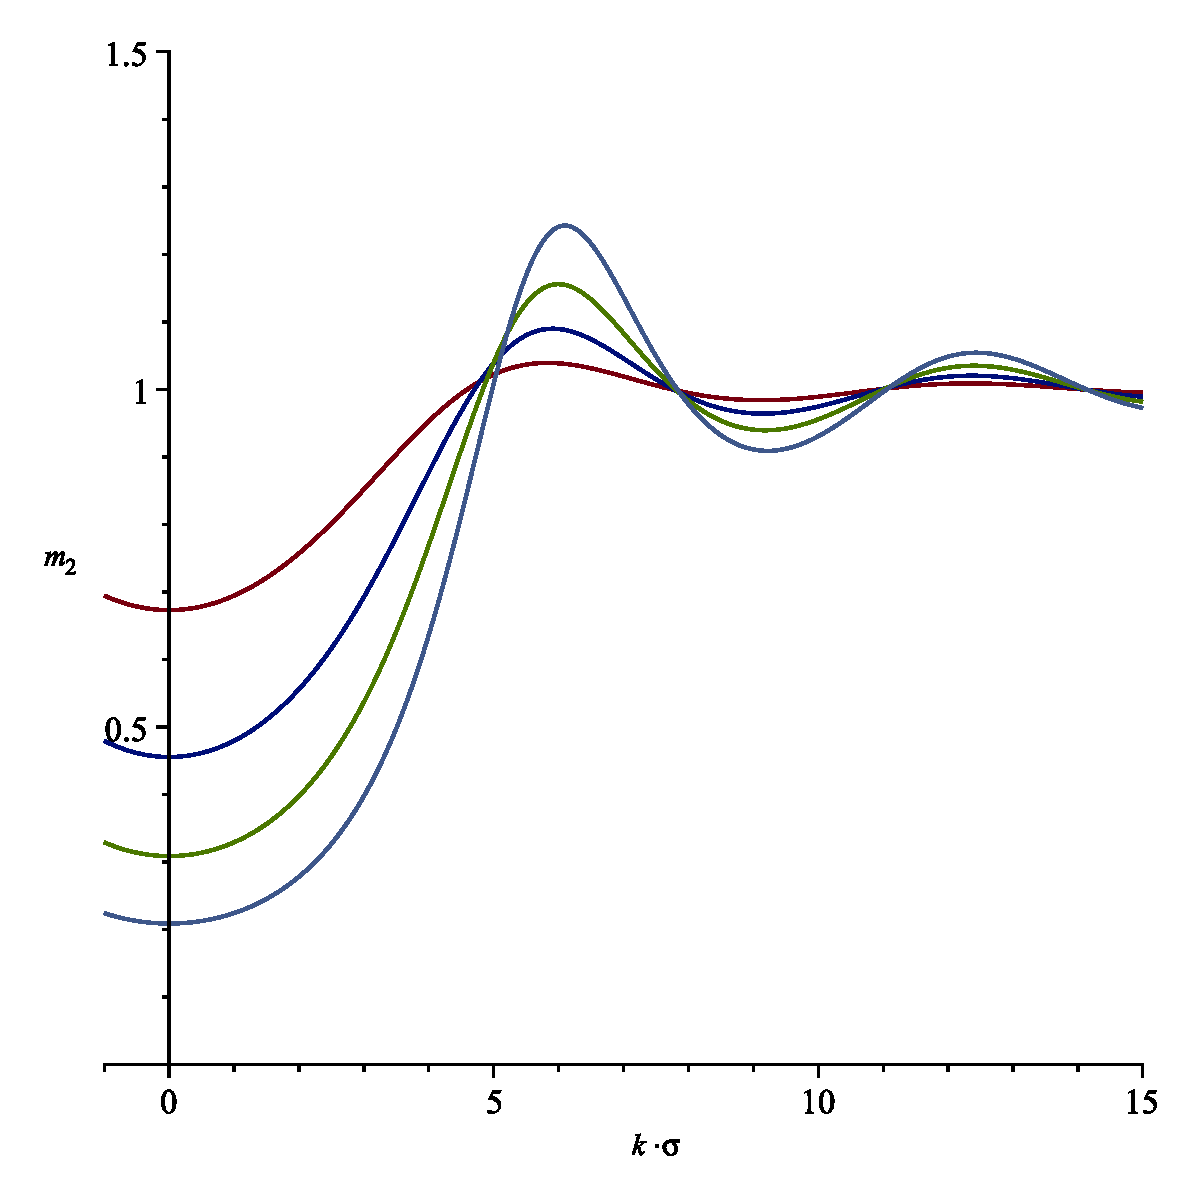
\includegraphics[width=0.45\textwidth,angle=0]{M2_as_function_of_k_at_different_eta} \hfill
	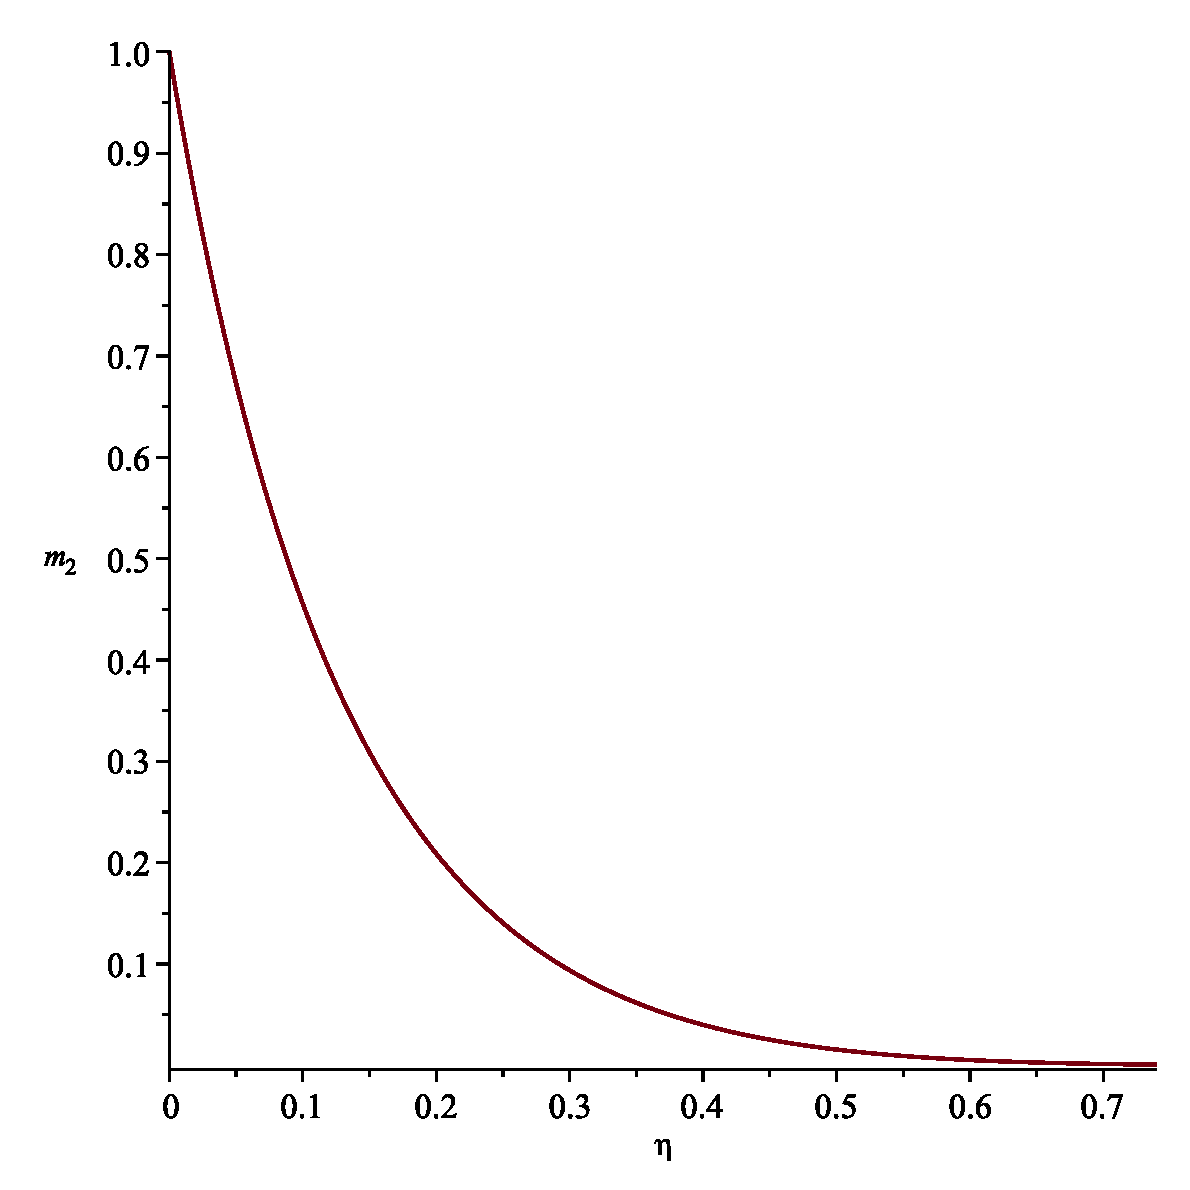
\includegraphics[width=0.45\textwidth,angle=0]{M2_as_function_of_eta_at_k_equals_0} \\
	\parbox{0.5\textwidth}{\caption{\label{m2_vs_k} Cumulant $\mathfrak{m}_2$ as a function of $k\sigma$ at different values of packing fraction $\eta$. $\eta = 0.05$, $\eta=0.1$, $\eta = 0.15$, and $\eta=0.2$.
	}} \hfill
	\parbox{0.45\textwidth}{\caption{\label{m2_vs_eta} Cumulant $\mathfrak{m}_2$ as a function of packing fraction $\eta$ at $\vb k = 0$
	}}
\end{figure}

The formulas for $\mathfrak{M}_3(\vb k, -\vb k, 0)$ and $\mathfrak{M}_4(\vb k, -\vb k, 0, 0)$ can be obtained from $\mathfrak{M}_2(\vb k, -\vb k)$ based on the recurrence relations for $n$-particle distribution functions $g_n$ found in~\cite{Schofield1966} (see Eq.~(A8) therein). Such formulas were obtained in~\cite{YukhJSP1995} (see Appendix B therein) and in our notation they read:
\begin{equation}
	\label{recur_m3_m2}
	\mathfrak{m}_3(\vb k, -\vb k) = \mathfrak{m}_2(0) 
	\left[
		\mathfrak{m}_2(\vb k) + \eta\frac{\partial\mathfrak{m}_2(\vb k)}{\partial\eta}
	\right],
\end{equation}

\begin{eqnarray}
	\label{recur_m4_m2}
	\mathfrak{m}_4(k, -k, 0) &=& \mathfrak{m}_2(0) 
	\left[
		\mathfrak{m}_2(k)\mathfrak{m}_2(0) + 3\eta\mathfrak{m}_2(0)\frac{\partial\mathfrak{m}_2(k)}{\partial\eta}
	\right.
	\nonumber\\
	&& \left. 
	+ \eta\mathfrak{m}_2(k)\frac{\partial\mathfrak{m}_2(0)}{\partial\eta} 
	+ \eta^2\frac{\partial\mathfrak{m}_2(0)}{\partial\eta} \frac{\partial\mathfrak{m}_2(k)}{\partial\eta}
	+ \eta^2\mathfrak{m}_2(0)\frac{\partial^2\mathfrak{m}_2(k)}{\partial\eta^2}
	\right]
\end{eqnarray}

\begin{figure}[htbp]
	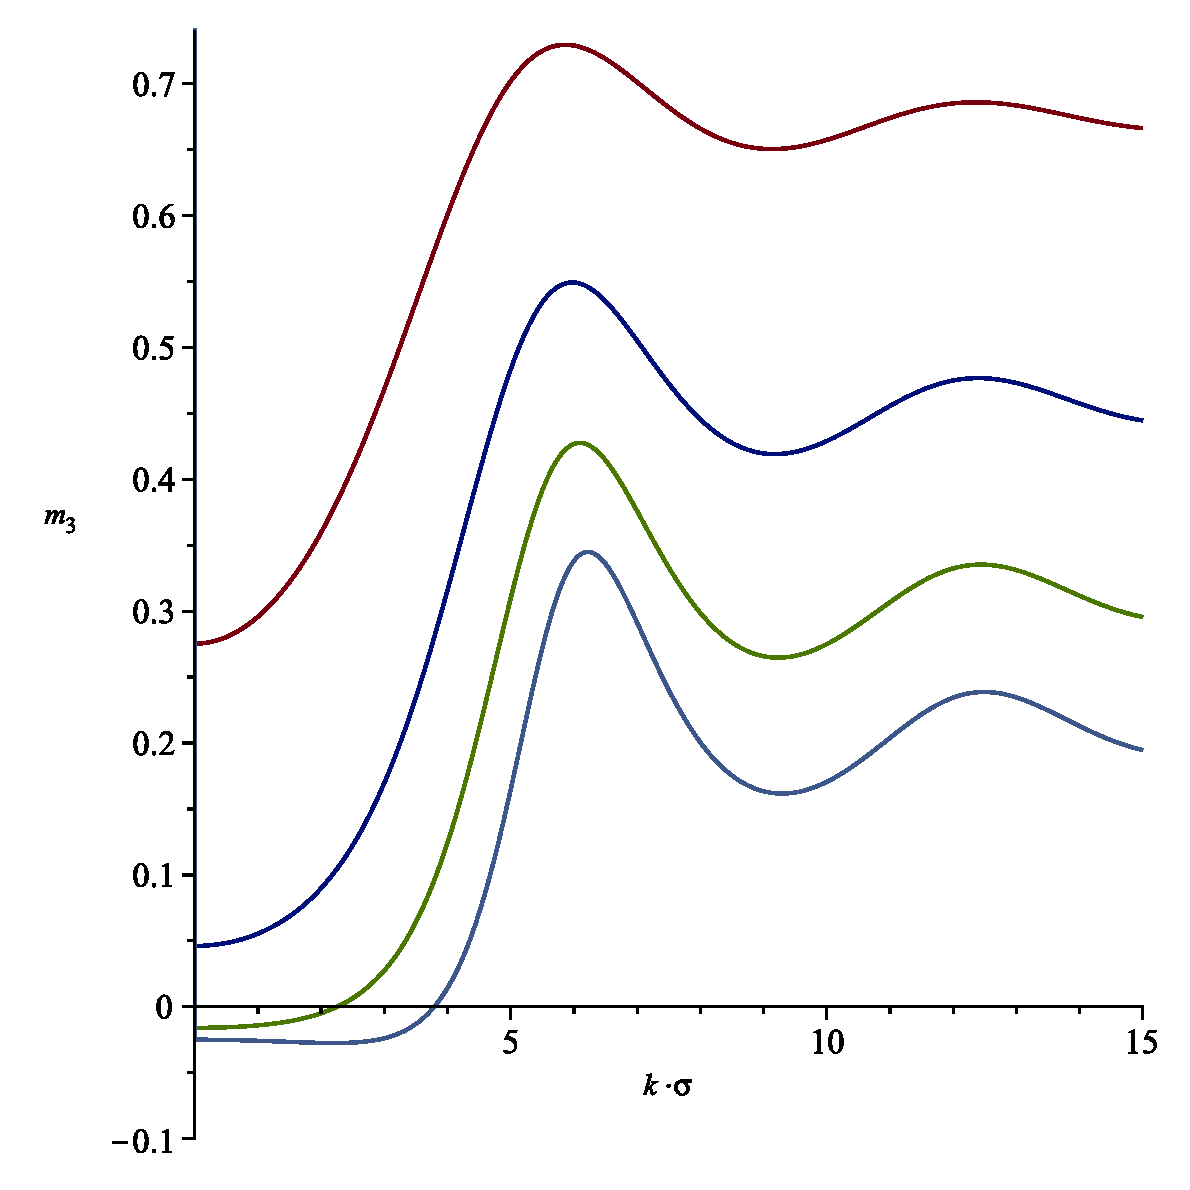
\includegraphics[width=0.45\textwidth,angle=0]{M3_as_function_of_k_at_different_eta} \hfill
	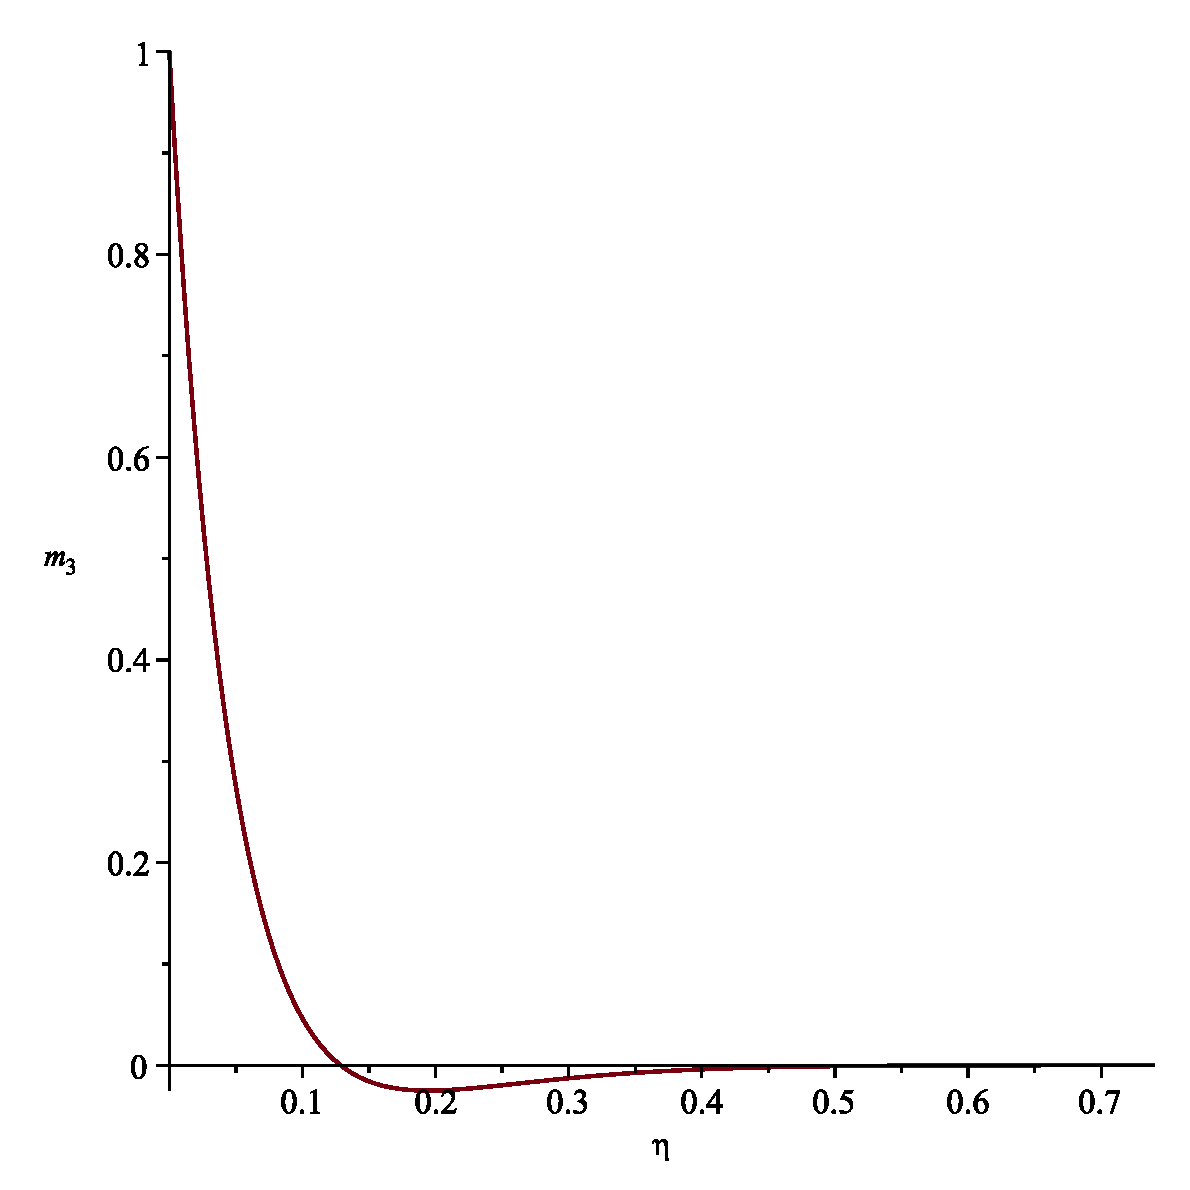
\includegraphics[width=0.45\textwidth,angle=0]{M3_as_function_of_eta_at_k_equals_0} \\
	\parbox{0.5\textwidth}{\caption{\label{m3_vs_k} Cumulant $\mathfrak{m}_3$ as a function of $k\sigma$ at different values of packing fraction $\eta$. $\eta = 0.05$, $\eta=0.1$, $\eta = 0.15$, and $\eta=0.2$.
	}} \hfill
	\parbox{0.45\textwidth}{\caption{\label{m3_vs_eta} Cumulant $\mathfrak{m}_3$ as a function of packing fraction $\eta$ at $\vb k = 0$
	}}
\end{figure}
\begin{figure}[htbp]
	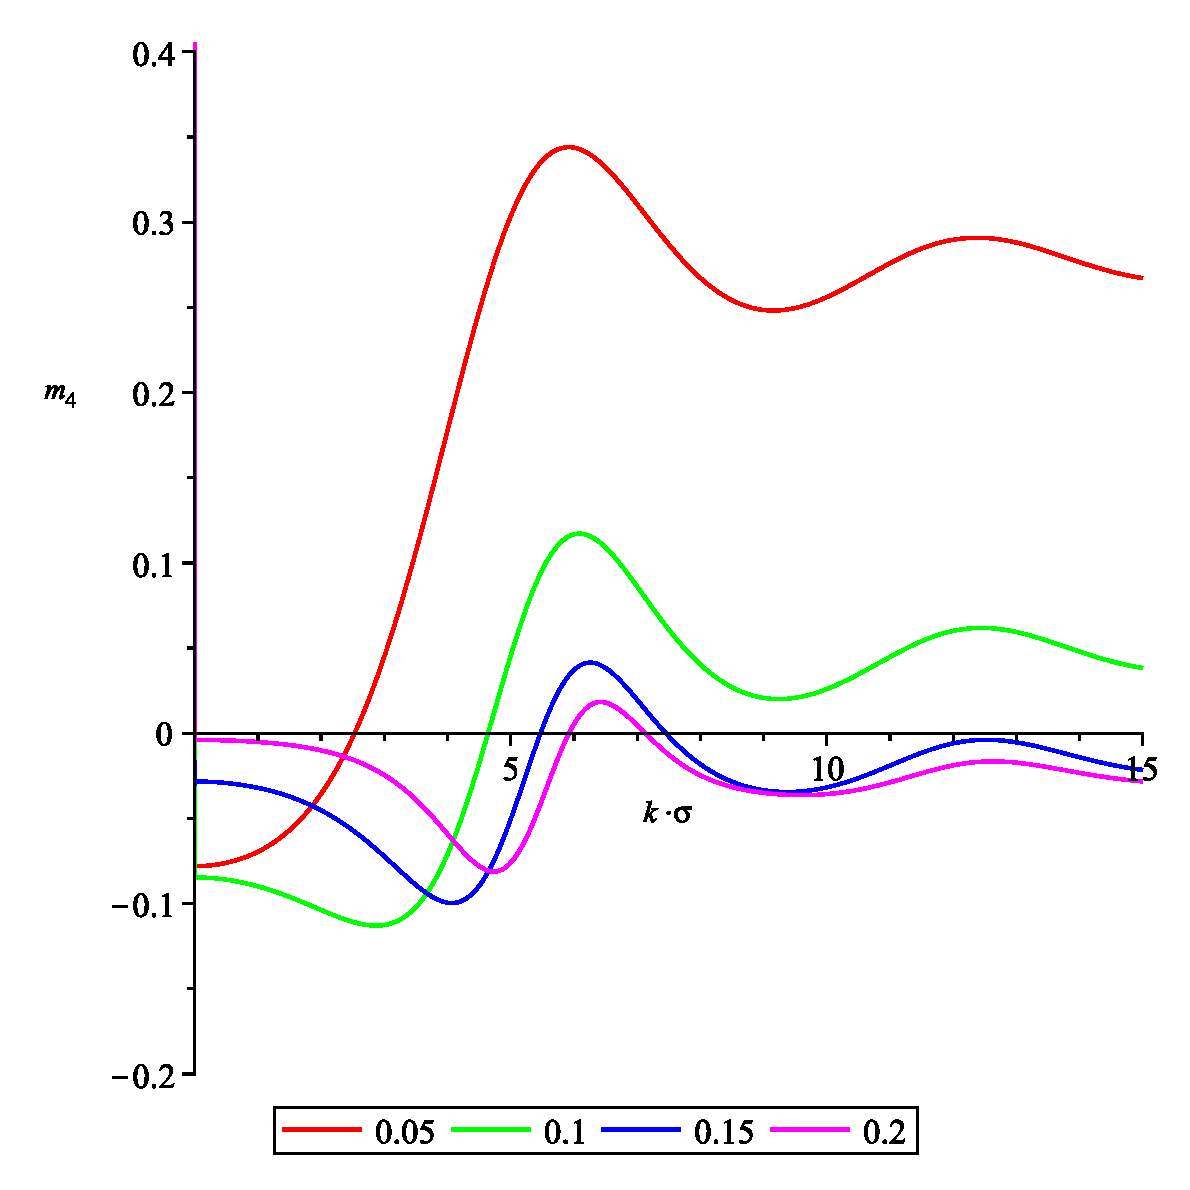
\includegraphics[width=0.45\textwidth,angle=0]{M4_as_function_of_k_at_different_eta} \hfill
	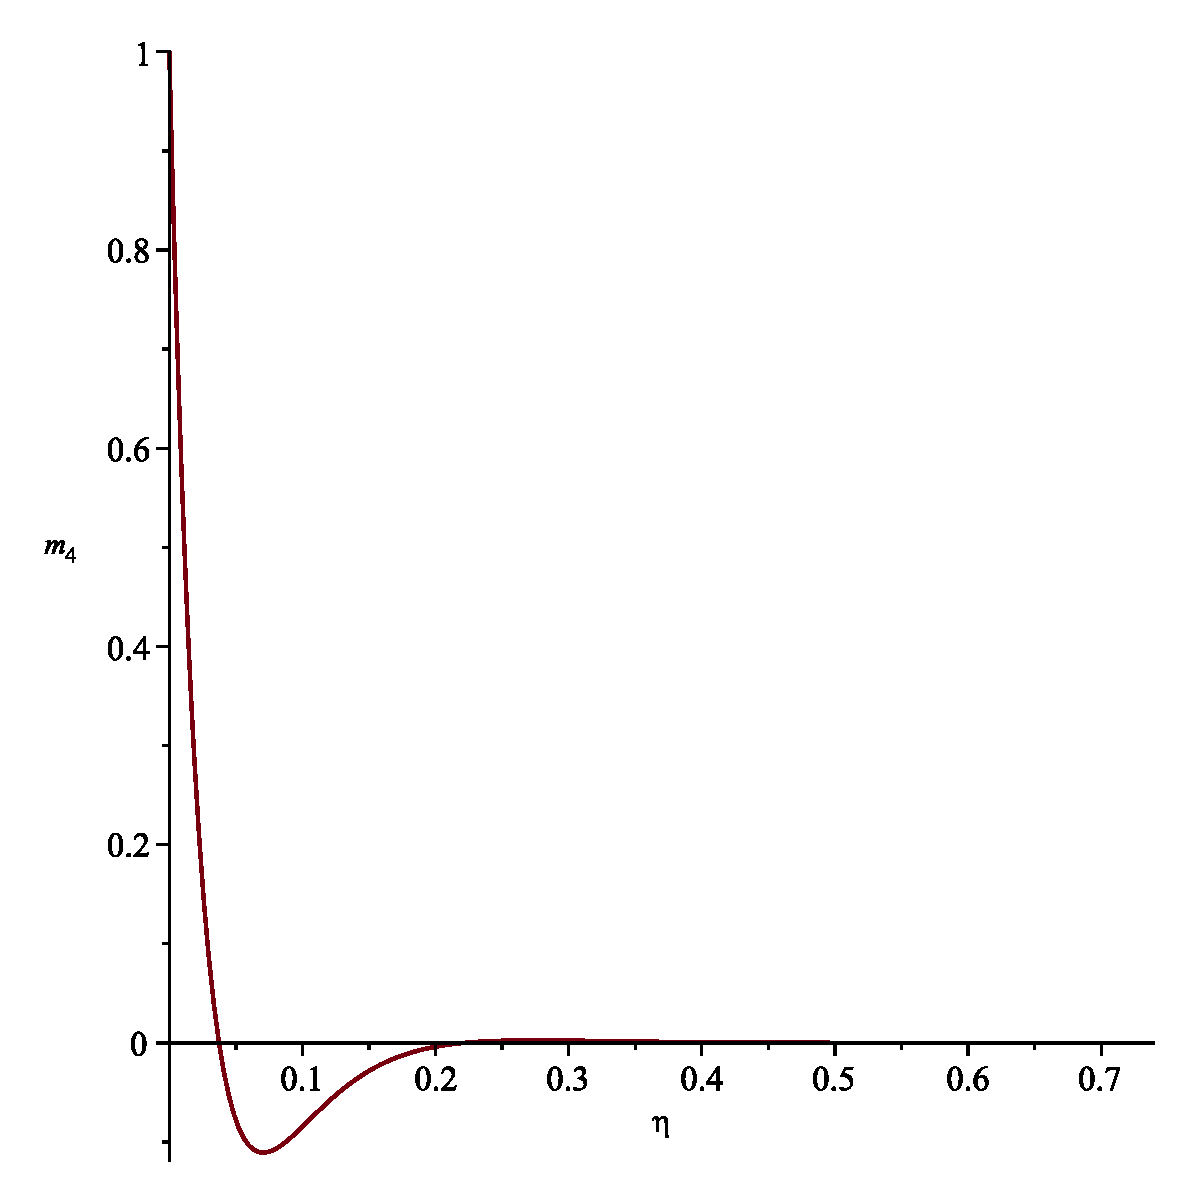
\includegraphics[width=0.45\textwidth,angle=0]{M4_as_function_of_eta_at_k_equals_0} \\
	\parbox{0.5\textwidth}{\caption{\label{m4_vs_k} Cumulant $\mathfrak{m}_4$ as a function of $k\sigma$ at different values of packing fraction $\eta$. $\eta = 0.05$, $\eta=0.1$, $\eta = 0.15$, and $\eta=0.2$.
	}} \hfill
	\parbox{0.45\textwidth}{\caption{\label{m4_vs_eta} Cumulant $\mathfrak{m}_4$ as a function of packing fraction $\eta$ at $\vb k = 0$
	}}
\end{figure}
In Figure~\ref{m3_vs_k} $\mathfrak{m}_3$ is shown as a function of $k\cdot\sigma$ at different values of $\eta$. In Figure~\ref{m3_vs_eta} $\mathfrak{m}_3$ is shown as a function of $\eta$ at $k=0$.
In Figure~\ref{m4_vs_k} $\mathfrak{m}_4$ is shown as a function of $k\cdot\sigma$ at different values of $\eta$. In Figure~\ref{m4_vs_eta} $\mathfrak{m}_4$ is shown as a function of $\eta$ at $k=0$.

\subsection{Cumulants at $\vb k_i = 0$}
At $\vb k_i = 0$ cumulants are expressed via the average number of particles in the reference system.
Here the final expressions are presented. They are obtained directly from~(\ref{m1_via_rho})--(\ref{m4_via_rho}) by substituting $\vb k_i=0$ and using $\hat{\rho}_0 = N$. Some alternative methods to calculate them are presented in Appendix~\ref{app:cumulant_calc_k_0}.
\begin{equation}
	\mathfrak{M}_1(0) = \langle N \rangle_0;
\end{equation}

\begin{equation}
	\mathfrak{M}_2(0,0) = \langle N^2 \rangle_0 - \langle N \rangle_0^2 = \langle (N - \langle N \rangle_0)^2 \rangle_0;
\end{equation}

\begin{eqnarray}
	\mathfrak{M}_3(0,0,0) &=& \langle N^3 \rangle_0 - 3 \langle N^2 \rangle_0 \langle N \rangle_0 +2\langle N \rangle_0^3
	\nonumber\\
	&=& \langle (N - \langle N \rangle_0)^3 \rangle_0;
\end{eqnarray}

\begin{eqnarray}
	\mathfrak{M}_4(0,0,0,0) &=& \langle N^4 \rangle_0 
	- 4\langle N^3 \rangle_0\langle N \rangle_0 
	+ 12\langle N^2 \rangle_0\langle N \rangle_0^2 
	- 3\langle N^2 \rangle_0^2 
	- 6\langle N \rangle_0^4
	\nonumber\\
	&=& \langle (N - \langle N \rangle_0)^4 \rangle_0 - 3 \langle (N - \langle N \rangle_0)^2 \rangle_0^2.
\end{eqnarray}

\section{Grand partition function in the representation of collective variables}
The grand partition partition function is now written as 
\begin{eqnarray}
	\label{gpf_1}
	\Xi &=& \Xi_0 \int \exp \left[h \rho_0 - \frac12
	\sum\limits_{\bf k} \alpha (k) \rho_{\bf k}\rho_{-{\bf k}} \right]
	\\
	&&
	\quad{}\times
	\exp (i2\pi \sum\limits_{\bf k} \omega_{\bf k} \rho_{\bf k} + \sum_{n\ge 1} \frac{(-i2\pi)^n}{n!}\sum_{\vb{k}_1,\dotsc,\vb{k}_n} {\mathfrak M}_n(\vb{k}_1,\dotsc,\vb{k}_n) \omega_{\vb k_1}\dotsc\omega_{\vb{k}_n})
	(d\omega) (d\rho) \nonumber
\end{eqnarray}
This expression was obtained in \cite{Yukh1990}, see Eq.(2.16).

The next step in calculation is to integrate over $\omega_{\vb k}$ with $\vb{k}>B$. This integration can be performed with Gaussian measure, i.e. the expressions in the exponent is restricted to the powers of $\omega$ not higher than 2. Let us denote the result of this integration by $\Xi_G$. Then the grand partition function takes the form:
\be
\Xi = \Xi_0\Xi_G\Xi_L
\ee
Here $\Xi_L$ denotes long-wave contributions to the GPF and is the object of our further investigation in this paper. The expression for $\Xi_L$ is following (see also Eq.(3.5) in \cite{Yukh1990}):
\begin{eqnarray}
	\label{gpf_l1}
	\Xi_L &=& \int \exp \left[h \rho_0 - \frac12
	\sum\limits_{\vb k \atop k\le B} \alpha (k) \rho_{\vb k}\rho_{-{\vb k}} \right]
	\\
	&&
	\quad{}\times
	\exp (i2\pi \sum\limits_{\vb k \atop k\le B} \omega_{\vb k} \rho_{\vb k} + \sum_{n\ge 1} \frac{(-i2\pi)^n}{n!}\sum_{\vb{k}_1,\dotsc,\vb{k}_n \atop k_i\le B} \tilde{\frak M}_n(\vb{k}_1,\dotsc,\vb{k}_n) \omega_{\vb k_1}\dotsc\omega_{\vb{k}_n})
	(d\omega)^{N_B} (d\rho)^{N_B} \nonumber
\end{eqnarray}
Here $\tilde{\frak M}_n$ denote renormalized cumulants ${\frak M}_n$ due to integration over $k>B$ [explicity expressions are needed?], and
\be
(d\omega)^{N_B} (d\rho)^{N_B} = \left(\prod_{\vb k\atop k\le B}d\omega_{\vb k}^c d\rho_{\vb k}^c d\omega_{\vb k}^s d\rho_{\vb k}^s \right) d\omega_0 d\rho_0
\ee

In the approximation of the $4th$ basic measure density, $\Xi_L$ is expressed as:
\be
\label{gpf_l3}
\Xi_L = \int (1 + D_4 + \frac12D_4^2 + \dotsc) W_4 (\rho;\omega) (d\rho)^{N_B}(d\omega)^{N_B}, 
\ee
where the measure density $W_4(\rho; \omega)$ is
\begin{eqnarray}
	\label{meas_dens_1}
	&& W_4(\rho;\omega) = \exp \left\{ h\rho_0
	- \frac12  \sum\limits_{{\vb k}\atop k\le B} \alpha(k) \rho_{\vb k} \rho_{-{\vb k}}
	+ i2\pi \sum\limits_{{\vb k} \atop k\le B} \omega_{\vb k} \rho_{\vb k} + \right.  \nonumber\\
	&& \left.+
	\sum\limits_{n=1}^4 \frac{(-i2\pi)^n}{n!} 
	\sum\limits_{\vb{k}_1,\dotsc,\vb{k}_n\atop{k_i \le B}} \tilde{\frak M}_n(\vb{k}_1,\dotsc,\vb{k}_n)
	\omega_{{\vb k}_1} \dots \omega_{{\vb k}_n} \right\}.
\end{eqnarray}
and the following notation is introduced:
\be
D_4 = \sum_{m>4}\frac{(-i2\pi)^m}{m!} \sum\limits_{\vb{k}_1,\dotsc,\vb{k}_m\atop{k_i \le B}}
\tilde{\frak M}_n(\vb{k}_1,\dotsc,\vb{k}_m)
\omega_{{\vb k}_1} \dots \omega_{{\vb k}_m}
\ee

The quantity $N_B$ is the number of variables to be integrated over. It is equal to the
number of values that the wave vector takes on in the sphere of radius B in reciprocal space. Let's assume that the wave-vector values are distributed uniformly, then
\be
\label{NB}
N_B = \frac{B^3}{6\pi^2}V.
\ee
To derive this equation, consider the following arguments. If we had a simple cubic lattice of spacing
$c$ in real space, the first Brillouin zone of it would be a simple cubic lattice in the reciprocal
space with spacing $2B'$, where $B'=\pi/c$. The number of values taken by wave vector in this zone
would be $N_{B} = V/c^3 = V(B'/\pi)^3.$ Under our assumption, the wave vector values are distributed
uniformly. Hence, the sphere of volume $\Omega$ in reciprocal space must contain the same number of wave
vector values as a cube of the same volume $\Omega$. Since $\Omega = (2B')^3 = \frac43\pi B^3,$ one finds that $B'^3=\frac{\pi}{6}B^3$ and, therefore, arrives at Eq.~(\ref{NB}). [Some references are needed here]

In the current investigation the following approximations are to be applied.

{\it Approximation 1.} $D_4$ is neglected in the expression (\ref{gpf_l3}) for $\Xi_L$;

{\it Approximation 2.} The difference between renormalized values of cumulants $\tilde{\frak M}_n$ and original cumulants $\frak M_n$ is ignored, so that:
\be
\tilde{\frak M}_n(\vb k^n) \approx \frak M_n(\vb k^n)
\ee

{\it Approximation 3.} The dependence of cumulants $\frak M_n$ on the wave vectors $\vb k_i$ is neglected, except for the dependence via $\delta$-functions
\be
\frak{M}_n({\vb k}^n) \approx \frak{M}_n(0^n) \delta_{\vb{k}_1 + \dotsc + \vb{k}_n}
\ee
where the following notation is used for simplicity: ${\vb k}^n\equiv {\vb k}_1, \dotsc, {\vb k}_n$.

With these approximations applied, one arrives at the following expressions:
\be
\label{gpf_l4}
\Xi_L = \int W_4 (\rho;\omega) (d\rho)^{N_B}(d\omega)^{N_B}, 
\ee
and
\begin{eqnarray}
	\label{meas_dens_2}
	W_4(\rho;\omega) &=& \exp \left\{ h\rho_0
	- \frac12  \sum\limits_{{\vb k}\atop k\le B} \alpha(k) \rho_{\vb k} \rho_{-{\vb k}}
	+ i2\pi \sum\limits_{{\vb k} \atop k\le B} \omega_{\vb k} \rho_{\vb k} \right.  \nonumber\\
	&& \left.+
	\sum\limits_{n=1}^4 \frac{(-i2\pi)^n}{n!} 
	{\frak M}_n(0^n)
	\sum\limits_{\vb{k}_1,\dotsc,\vb{k}_n\atop{k_i \le B}}
	\delta_{\vb{k}_1 + \dotsc + \vb{k}_n} 
	\omega_{{\vb k}_1} \dots \omega_{{\vb k}_n} \right\}.
\end{eqnarray}
See also Eqs.~(3.12),~(3.13) in \cite{Yukh1990}.

The expression \ref{meas_dens_2} for the $4$-th measure density contains non-zero terms in all powers of $\omega$ up to 4. Let's eliminate the coefficient next to the 3-rd power in $\omega$. For this, the following change of variables is performed:
\be
\omega_0 = \omega'_0 + \frac{\frak M_3}{(i2\pi) \frak M_4}
\ee
From now on, we will understand $\frak M_n$ as $\frak{M}_n(0^n)$ where it is not ambiguous. One should remember that $\frak M_n$ are still dependent on the packing fraction $\eta$.
The 4-th measure density $W_4(\rho; \omega)$ takes the form:

\begin{eqnarray}
	\label{meas_dens_3}
	W_4(\rho;\omega) &=& \exp \left\{\frak M_0 + (h + \frak M_3/\frak M_4)\rho_0
	- \frac12  \sum\limits_{{\vb k}\atop k\le B} \alpha(k) \rho_{\vb k} \rho_{-{\vb k}}
	- i2\pi \tilde{\frak M}_1 \omega_0 + \right.  \nonumber\\
	&&
	+ i2\pi \sum\limits_{{\vb k} \atop k\le B} \omega_{\vb k} \rho_{\vb k}
	+ \frac{(-i2\pi)^2}{2!}\tilde{\frak M}_2 \sum\limits_{{\vb k} \atop k\le B} \omega_{\vb k} \omega_{-\vb k}
	\nonumber\\
	&& \left. +
	\frac{(-i2\pi)^4}{4!} 
	{\frak M}_4
	\sum\limits_{\vb{k}_1,\dotsc,\vb{k}_4\atop{k_i \le B}}
	\delta_{\vb{k}_1 + \dotsc + \vb{k}_4} 
	\omega_{{\vb k}_1} \dots \omega_{{\vb k}_4} \right\}
\end{eqnarray}
with
\be
\frak M_0 = -\frac{\frak M_1 \frak M_3}{\frak M_4} + \frac{\frak M_2 \frak M_3^2}{2 \frak M_4^2}
- \frac{\frak M_3^4}{8\frak M_4^3},
\ee

\be
\tilde{\frak M}_1 = \frak M_1 -\frac{\frak M_2 \frak M_3}{\frak M_4} + \frac{\frak M_3^3}{3\frak M_4^2},
\ee

\be
\tilde{\frak M}_2 = \frak M_2 - \frac{\frak M_3^2}{2 \frak M_4}.
\ee
In (\ref{meas_dens_3}) the prime at $\omega_0$ is omitted.

We also want to eliminate the term at $\omega_0$. This is achieved by the change of variables
\be
\rho_0 = \rho'_0 + \tilde{\frak M}_1.
\ee
The expression for $W_4(\rho; \omega)$ becomes
\begin{eqnarray}
	\label{meas_dens_4}
	W_4(\rho;\omega) &=& \exp \left\{\tilde{\frak M}_0 + \mu^*\rho_0
	- \frac12  \sum\limits_{{\vb k}\atop k\le B} \alpha(k) \rho_{\vb k} \rho_{-{\vb k}} \right.  \nonumber\\
	&&
	+ i2\pi \sum\limits_{{\vb k} \atop k\le B} \omega_{\vb k} \rho_{\vb k}
	+ \frac{(-i2\pi)^2}{2!}\tilde{\frak M}_2 \sum\limits_{{\vb k} \atop k\le B} \omega_{\vb k} \omega_{-\vb k}
	\nonumber\\
	&& \left. +
	\frac{(-i2\pi)^4}{4!} 
	{\frak M}_4
	\sum\limits_{\vb{k}_1,\dotsc,\vb{k}_4\atop{k_i \le B}}
	\delta_{\vb{k}_1 + \dotsc + \vb{k}_4} 
	\omega_{{\vb k}_1} \dots \omega_{{\vb k}_4} \right\}
\end{eqnarray}
with
\begin{equation}
\label{tilde_frak_M0}
\tilde{\frak M}_0 = \frak M_0 + (h + {\frak M_3}/{\frak M_4})\tilde{\frak M}_1 - \frac{\alpha(0)}{2}\tilde{\frak M}_1^2
\end{equation}

\begin{equation}
	\label{mu_star}
	\mu^* = h + {\frak M_3}/{\frak M_4} + \alpha(0)\tilde{\frak M}_1
\end{equation}
In (\ref{meas_dens_4}) the prime at $\rho_0$ is omitted.

We can compare the expression~(\ref{meas_dens_4}) with Eq.~(3.14) from \cite{Yukh1990}, Eq.~(12) from \cite{YukhJSP1995}, and Eq.~(3.5) from \cite{Yukh2013}.

\begin{table}[h]
	\caption{The zero values of the cumulant $\mathfrak{M_4}$. $\mathfrak{M_4} < 0$ for $\eta_{min} < \eta < \eta_{max}$.}
	\label{tab:cum_m4_zeros}
	\begin{center}
		\begin{tabular}{|c|c|c|}
			%\begin{tabular}{cccccccccc}
			\hline
			Approximation & $\eta_{min}$ & $\eta_{max}$ \\
			\hline
			Percus-Yevick, compressibility equation \quad & 0.037346 \quad & 0.221675 \quad \\
			Percus-Yevick, virial equation          & 0.037673 & 0.233899 \\
			Carnahan-Starling                       & 0.037455 & 0.225572 \\
			Ree-Hoower                              & 0.037423 & 0.224260 \\
			\hline
		\end{tabular}
	\end{center}
\end{table}

\begin{figure}[htbp]
	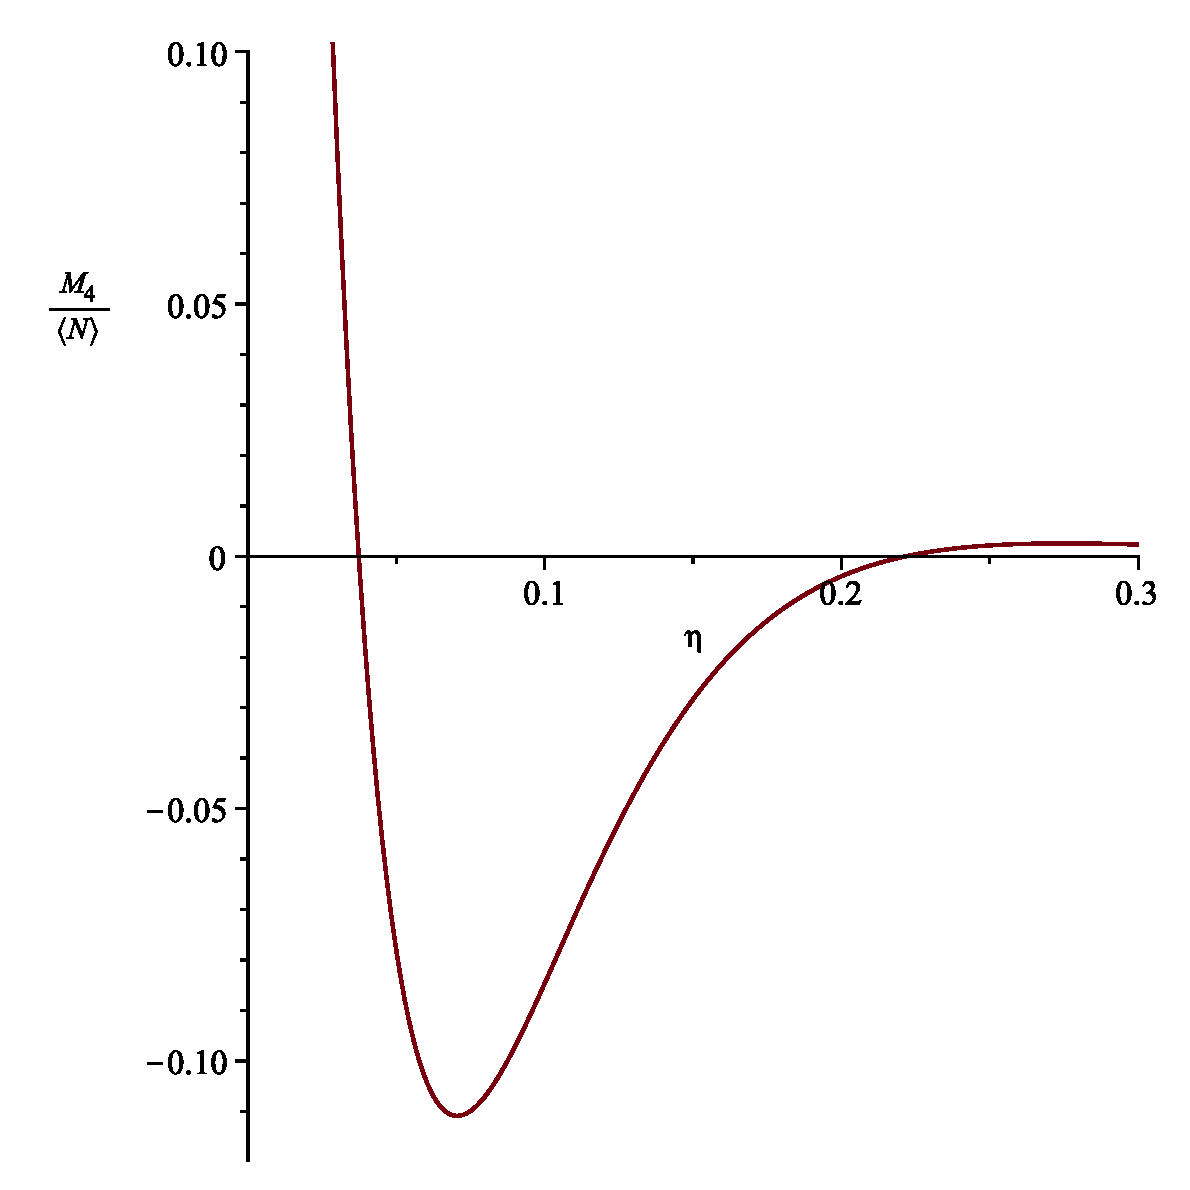
\includegraphics[width=0.7\textwidth,angle=0]{M4_at_k_equals_0_as_function_of_eta}
	\caption{Cumulant $\frak M_4$ as a function of packing fraction $\eta$ at $\vb k_i = 0$.}
	\label{m4_fig1}
\end{figure}

The first thing to note in Eq.~(\ref{meas_dens_4}) is that the integral for $\Xi_L$ in~(\ref{gpf_l4}) converges only for $\frak M_4 < 0$. The values of $\mathfrak M_4$ are negative only in some range of $\eta$. Table~{\ref{tab:cum_m4_zeros}} summarizes numerical solutions for the equation $\mathfrak{M_4}=0$ in a few approximations. Thus one can conclude that the 4-th measure density $W_4(\rho; \omega)$ is applicable only in this range of packing fraction $\eta$. We are going to work in range $0.04 \le \eta \le 0.22$. The dependence of $\frak M_4$ on $\eta$ is presented in Figure~\ref{m4_fig1}.

\subsection{Integration over $\omega$.}
Let's perform integration over $\omega$ in~(\ref{gpf_l4}), using~(\ref{meas_dens_4}) for $W_4(\rho; \omega)$. First let's single out the integral over $\omega$
\begin{eqnarray}
	J(\rho) &=& \int \exp \left(
	{\rm i}2\pi \sum\limits_{{\vb k} \atop k\le B} \omega_{\vb k} \rho_{\vb k}
	+ \frac{(-i2\pi)^2}{2!}\tilde{\frak M}_2 \sum\limits_{{\vb k} \atop k\le B} \omega_{\vb k} \omega_{-\vb k}
	\right.
	\nonumber\\
	&& \left. +
	\frac{(-i2\pi)^4}{4!} 
	{\frak M}_4
	\sum\limits_{\vb{k}_1,\dotsc,\vb{k}_4\atop{k_i \le B}}
	\delta_{\vb{k}_1 + \dotsc + \vb{k}_4} 
	\omega_{{\vb k}_1} \dots \omega_{{\vb k}_4} \right) ({\rm d} \omega)^{N_B}
\end{eqnarray}
To factorize this integral, perform the following change of variables
\begin{equation}
	\tilde{\omega}_{\vb l} = \frac{1}{\sqrt{N_B}}\sum_{\substack{\vb k \\ k \leq B}} \omega_{\vb k} {\rm e}^{-{\rm i}\vb k \vb l}
	, \quad \tilde{\rho}_{\vb l} = \frac{1}{\sqrt{N_B}} \sum_{\substack{\vb k \\ k \leq B}} \rho_{\vb k} {\rm e}^{{\rm i}\vb k \vb l}.
\end{equation}
The following relations are valid:
\begin{equation}
	\sum_{\vb l} \tilde{\omega}_{l} \tilde{\rho}_{\vb l} = \frac{1}{N_B} \sum_{\vb l} \sum_{\vb k} \omega_{\vb k} \sum_{\vb k'} \rho_{\vb k'} {\rm e}^{-{\rm i} (\vb k - \vb k') \vb l} = \sum_{\vb k} \omega_{\vb k} \rho_{\vb k},
\end{equation}
\begin{eqnarray}
	&&\sum_{\vb l}\tilde{\omega}_{\vb l}^2 = \sum_{\vb k}\omega_{\vb k} \omega_{-\vb k},
	\\
	&&N_B \sum_{\vb l}\tilde{\omega}_{\vb l}^4 = \sum\limits_{\substack{\vb{k}_1,\dotsc,\vb{k}_4 \\ {k_i \le B}}}
	\delta_{\vb{k}_1 + \dotsc + \vb{k}_4} 
	\omega_{{\vb k}_1} \dots \omega_{{\vb k}_4}
\end{eqnarray}
where the following expression for the Kronecker's $\delta$-symbol is used:
\begin{equation}
	\delta_{\vb k} = \frac{1}{N_B}\sum_{\vb l} {\rm e}^{-{\rm i} \vb k \vb l}.
\end{equation}
The sum over $\vb l$ should be understood as running over $N_B$ values in real space corresponding to the wave-vector values $\vb k, k\leq B$.

The element of integration is changed as following:
\begin{equation}
	{\rm d} \omega_0 \prod'_{\substack{\vb k \\ k\leq B}} {\rm d} \omega_{\vb k}^c {\rm d}\omega_{\vb k}^s = j \prod_{\vb l} {\rm d} \tilde{\omega}_{\vb l}
\end{equation}
where $j$ is the Jacobian of transition from $\omega_{\vb k}$ to $\tilde{\omega}_{\vb l}.$

Since the approximation of the 4-th measure density is applicable only when $\mathfrak{M_4}$ is negative, we will write the following expressions using the absolute value of this cumulant. 
Thus, the factorized expression for the integral over $\omega$ is
\begin{equation}
	J(\rho) = j\prod_{\vb l} 
	\int \exp({\rm i}2\pi \tilde{\omega}_{\vb l} \tilde{\rho}_{\vb l} - \frac{(2\pi)^2}{2} \tilde{\mathfrak{M}}_2 \tilde{\omega}_{\vb l}^2 - \frac{(2\pi)^4}{4!}N_B \abs{\mathfrak{M}_4} \tilde{\omega}_{\vb l}^4)
	{\rm d}\tilde{\omega}_{\vb l}.
\end{equation}
If we denote the integral as
\begin{equation}
	J_{\vb l}(\tilde{\rho}_{\vb l}) = \int \exp({\rm i}2\pi \tilde{\omega}_{\vb l} \tilde{\rho}_{\vb l} 
	- \frac{(2\pi)^2}{2} \tilde{\mathfrak{M}}_2 \tilde{\omega}_{\vb l}^2 - \frac{(2\pi)^4}{4!}N_B \abs{\mathfrak{M}_4} \tilde{\omega}_{\vb l}^4)
	{\rm d}\tilde{\omega}_{\vb l}
\end{equation}
then the result of integration can be presented in the following form
\begin{equation}
	J(\rho) = j\prod_{\vb l}{\rm e}^{a_0} \exp(-\sum_{n\geq 1} \frac{a_n}{n!}\tilde{\rho}_{\vb l}^n)
\end{equation}
where coefficients $a_n$ are found by the following formulae
\begin{equation}
	a_n = - \left(\frac{\partial^n \ln J_{\vb l}(\tilde{\rho}_{\vb l})}{\partial \tilde{\rho}_{\vb l}^n}\right)_{\tilde{\rho}_{\vb l}=0}.
\end{equation}

First, let's calculate ${\rm e}^{a_0}$
\begin{equation}
	Q(\tilde{\mathfrak{M}}_2, \mathfrak{M}_4) \equiv {\rm e}^{a_0} = \int_{-\infty}^{\infty} 
	\exp(- \frac{(2\pi)^2}{2} \tilde{\mathfrak{M}}_2 \tilde{\omega}_{\vb l}^2 - \frac{(2\pi)^4}{4!}N_B \abs{\mathfrak{M}_4} \tilde{\omega}_{\vb l}^4) 
	{\rm d} \tilde{\omega}_{\vb l}.
\end{equation}
Using the following representation for the Weber parabolic cylinder function $U(a,x)$
	\begin{equation}
	\label{parab_cylinder_t4}
	U(a,x) = \frac{2}{\Gamma(a+\frac{1}{2})}{\rm e}^{-\frac{x^2}{4}} \int_{0}^{\infty}t^{2a}\exp\left(-xt^2 - \frac{1}{2}t^4\right) {\rm d} t
\end{equation}
one obtains:
\begin{equation}
	\label{quantity_Q}
	Q(\tilde{\mathfrak{M}}_2, \mathfrak{M}_4) = \frac{1}{2\sqrt{\pi}} \left(\frac{12}{N_B \abs{\mathfrak{M}_4}}\right)^{1/4} {\rm e}^{y^2/2} U(0,y)
\end{equation}
where 
\begin{equation}
	y = \left( \frac{3 \tilde{\mathfrak{M}_2^2}}{N_B \abs{\mathfrak{M}_4}}\right)^{1/2}.
\end{equation}

Now, let's calculate $a_2$.

For $a_2$ the result is
\begin{equation}
	a_2 = \left(\frac{3}{N_B \abs{\mathfrak{M}_4}}\right)^{1/2} U(y),
\end{equation}
where 
\begin{equation}
	U(y) = \frac{U(1,y)}{U(0,y)}.
\end{equation}

For $a_4$ the result is
\begin{equation}
	a_4 = \frac{3}{N_B \abs{\mathfrak{M}_4}}\left(3U^2(y) -3 \frac{U(2,y)}{U(0,y)}\right) = 
	\frac{3}{N_B \abs{\mathfrak{M}_4}} \phi(y)
\end{equation}
where 
\begin{equation}
	\phi(y) = 3U^2(y) + 2yU(y) - 2.
\end{equation}
In the above equation we used the following recurrence relation for the parabolic cylinder function $U$:
\begin{equation}
	3U(2,y) = -2yU(1,y) + 2U(0,y).
\end{equation}

The quantity $J(\rho)$ takes the form
\begin{equation}
	J(\rho) = j Q(\tilde{\mathfrak{M}_2}, \mathfrak{M}_4)^{N_B}
	\exp(-\frac{a_2}{2}\sum_{\substack{\vb k \\ k \leq B}} \rho_{\vb k}\rho_{-{\vb k}} 
	- \frac{a_4}{N_B 4!} \sum_{\substack{\vb k_1, \dotsc, \vb k_4 \\ k_i \leq B}} \rho_{\vb k_1} \dotsc \rho_{\vb k_4} \delta_{\vb{k}_1 + \dotsc + \vb{k}_4} )
\end{equation}
where the following equations were taken into account
\begin{eqnarray}
	&&\sum_{\vb l}\tilde{\rho}_{\vb l}^2 = \sum_{\vb k}\rho_{\vb k} \rho_{-\vb k},
	\\
	&&\sum_{\vb l}\tilde{\rho}_{\vb l}^4 = \frac{1}{N_B}\sum\limits_{\substack{\vb{k}_1,\dotsc,\vb{k}_4 \\ {k_i \le B}}}
	\delta_{\vb{k}_1 + \dotsc + \vb{k}_4} 
	\rho_{{\vb k}_1} \dots \rho_{{\vb k}_4}
\end{eqnarray}

Finally, the quantity $\Xi_L$ takes the form
\begin{equation}
	\Xi_L = jQ(\tilde{\mathfrak{M}_2}, \mathfrak{M}_4)^{N_B} \exp(\tilde{\mathfrak{M}}_0) \Xi_L^{(1)}
\end{equation}
where $Q(\tilde{\mathfrak{M}_2}, \mathfrak{M}_4)$ is given by~(\ref{quantity_Q}), $N_B$ by~(\ref{NB}), $\tilde{\mathfrak{M}_0}$ by~(\ref{tilde_frak_M0}), and $\Xi_L^{(1)}$ is defined as follows
\begin{equation}
	\label{Xi_L}
	\Xi_L^{(1)} = \int \exp(\mu^* \rho_0 - \frac{1}{2} \sum_{\substack{\vb k \\ k \leq B}} d(k) \rho_{\vb k} \rho_{-\vb k} - \frac{a_4}{4! N_B} \sum_{\substack{\vb k_1, \dotsc, \vb k_4 \\ k_i \leq B}} \rho_{\vb k_1} \dotsc \rho_{\vb k_4} \delta_{\vb{k}_1 + \dotsc + \vb{k}_4} ) ({\rm d} \rho)^{N_B}
\end{equation}
where $\mu^*$ is given by~(\ref{mu_star}), and 
\begin{equation}
	d(k) = a_2 + \alpha(k),
\end{equation}
where $\alpha(k)$ is given by~(\ref{def:h}).

\subsection{Coefficients of the effective Hamiltonian}
The argument $y$ of functions entering different expressions in the previous subsection is itself a function of $\eta$ and $B\sigma$. Let's show this.
\begin{equation}
	y=\left(\frac{3\tilde{\mathfrak{M}}_2^2}{N_B \abs{\mathfrak{M}_4}}\right)^{1/2} = \left(\frac{\langle N \rangle_0}{N_B}\right)^{1/2} \left(\frac{3\tilde{\mathfrak{m}}_2^2}{\abs{\mathfrak{m}_4}}\right)^{1/2},
\end{equation}
where the following notation is introduced
\begin{equation}
	\tilde{\mathfrak{m}}_2 = \mathfrak{m}_2 - \frac{\mathfrak{m}_3^2}{2\mathfrak{m}_4}.
\end{equation}
In the expression for $y$ the second multiplier depends only on $\eta$. Let's take a look at the first multiplier. Taking into account~(\ref{NB}), one has
\begin{equation}
	\frac{\langle N \rangle_0}{N_B} = \frac{\langle N \rangle_0}{V} \frac{6\pi^2}{B^3} = \frac{\langle N \rangle_0}{V}\sigma^3 \frac{6\pi^2}{(B\sigma)^3} = \frac{\pi}{6}\frac{\langle N \rangle_0}{V}\sigma^3 \frac{36\pi}{(B\sigma)^3} = \eta \frac{36\pi}{(B\sigma)^3}.
\end{equation}
The quantity $B\sigma$ is dimensionless but ist value depends on how $B$ is selected. Based on the previous works [References are needed], the condition for selecting $B$ is $\hat{\Phi}_{k=B} = 0.$ This condition impose some restrictions on the attractive part of the interaction potential, in particular that $\hat{\Phi}_0 < 0.$ However, section of the potential in the form of Eq.~(\ref{short-range-potential}) obeys this condition very well. 

The explicit expression for the Fourier component of such potential is the following
\begin{eqnarray}
	\hat{\Phi}_k &=& -16\pi \varepsilon \alpha^3 
	\left\{
		\frac{1}{1+k^2\alpha^2}\left(\frac{\sigma}{\alpha} + \frac{2}{1+k^2\alpha^2}\right) \cos(k\sigma)
	\right.
	\nonumber\\
	&& \left.
	 -\frac{1}{4 + k^2\alpha^2} \left(\frac{\sigma}{\alpha} + \frac{4}{4 + k^2\alpha^2}\right) \cos(k\sigma)
	 \right.
	 \nonumber \\
	&& \left.
	+ \frac{\sigma/\alpha}{1 + k^2\alpha^2} \left(\frac{\sigma}{\alpha} + \frac{1 - k^2\alpha^2}{1 + k^2 \alpha^2}\right) \frac{\sin(k\sigma)}{k\sigma}
	\right.
	\nonumber\\
	&& \left.
	- \frac{\sigma/\alpha}{4 + k^2\alpha^2} \left(2\frac{\sigma}{\alpha} + \frac{4 - k^2\alpha^2}{4 + k^2\alpha^2}\right) \frac{\sin(k\sigma)}{k\sigma}
	\right\}.
\end{eqnarray}
In this expression it is already taken into account that
\begin{equation}
	\sigma = R_0 - \alpha\ln(2).
\end{equation}

\begin{figure}[htbp]
	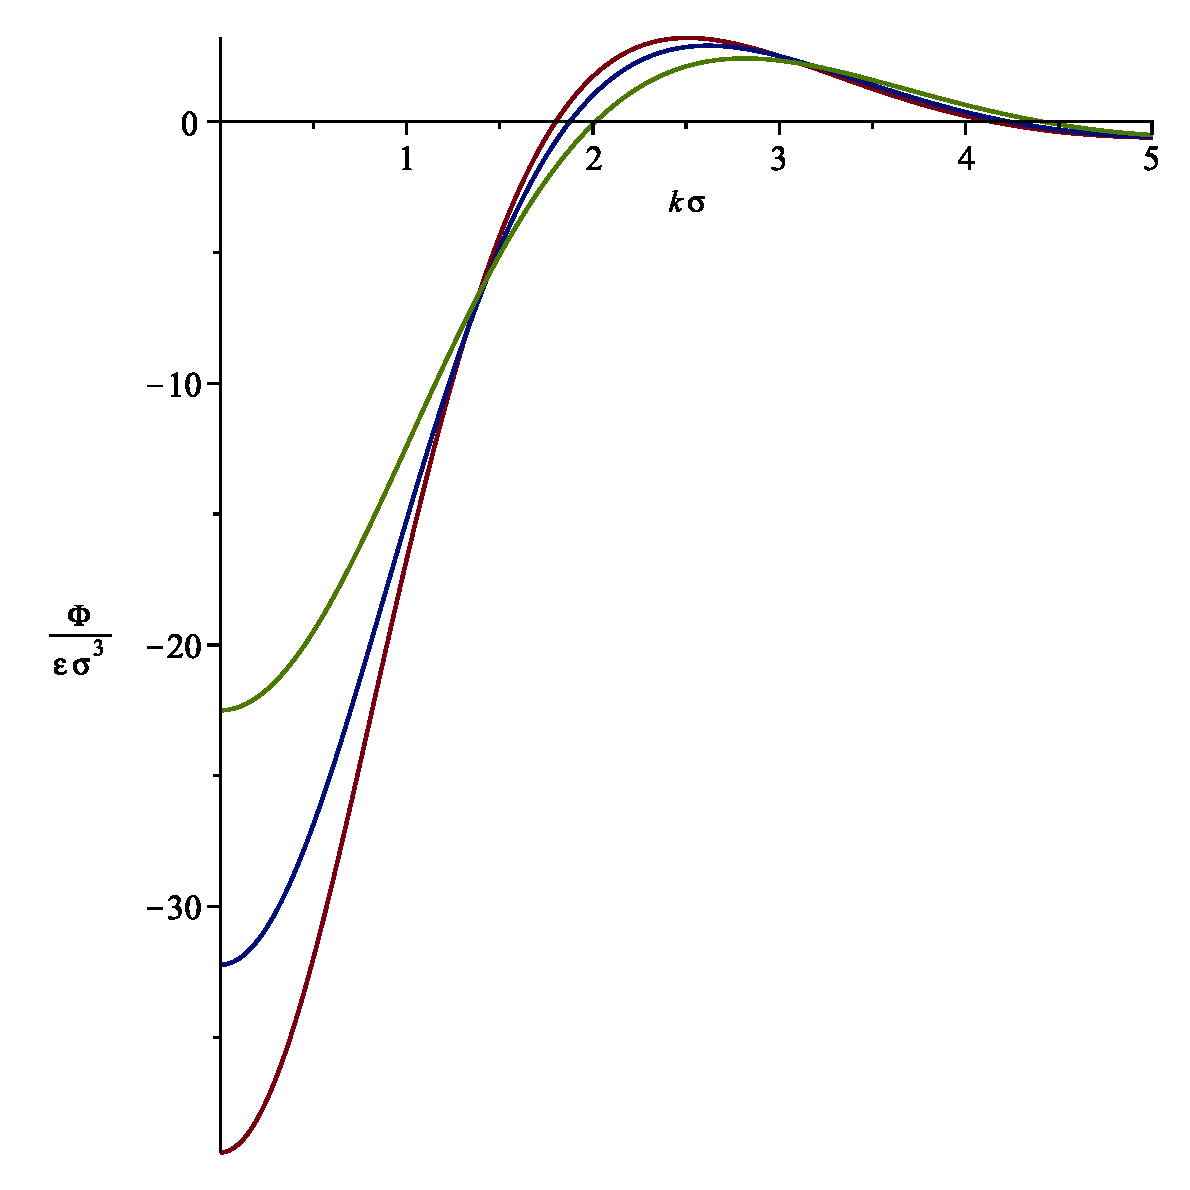
\includegraphics[width=0.45\textwidth,angle=0]{fourier_for_different_parameter_values} \hfill
	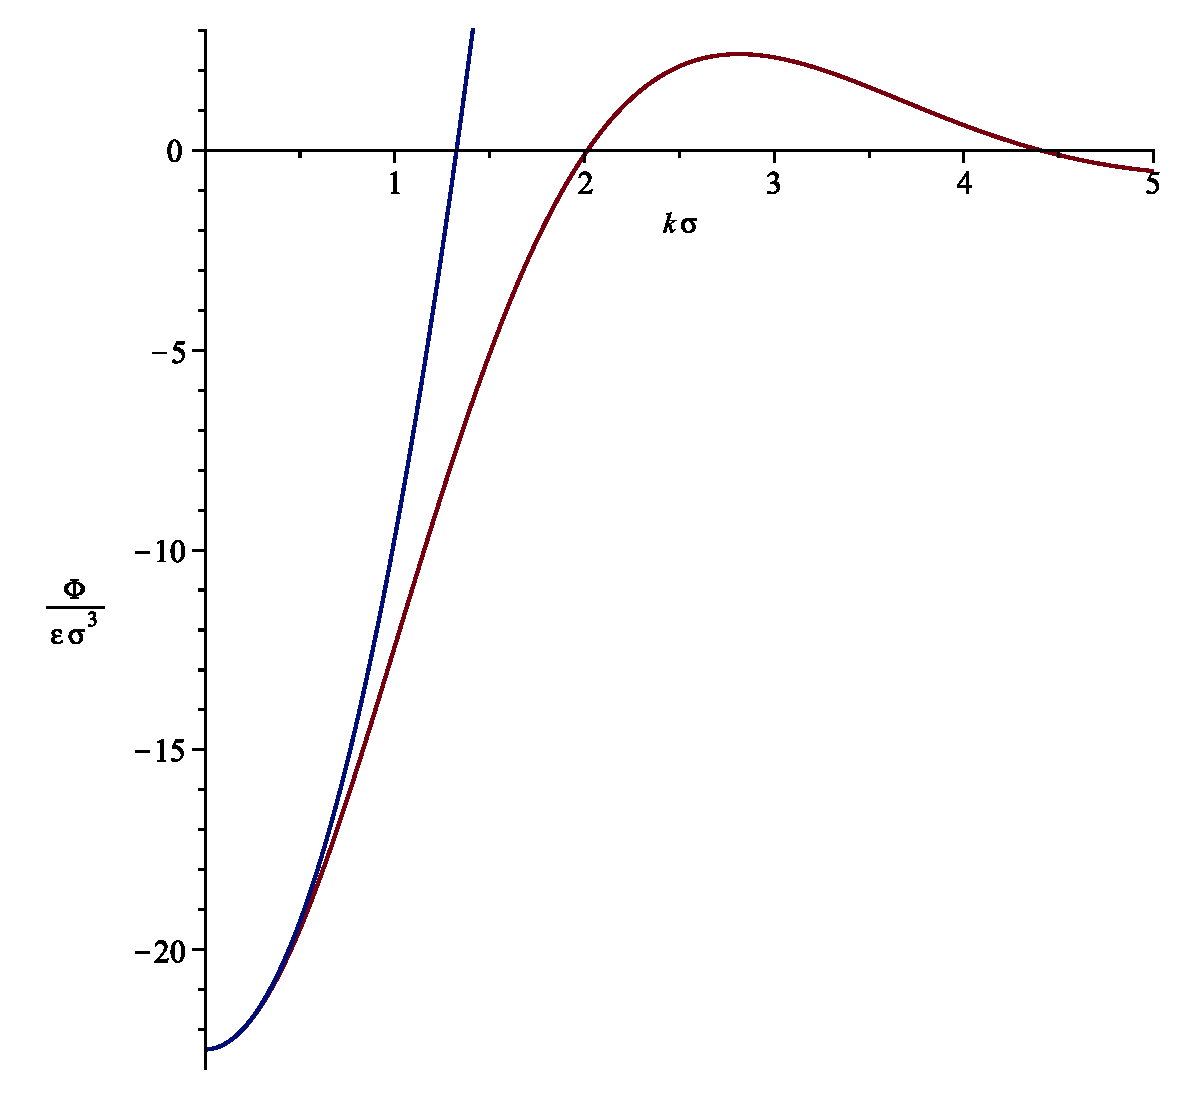
\includegraphics[width=0.45\textwidth,angle=0]{fourier_and_parabolic_potential} \\
	\parbox{0.5\textwidth}{\caption{\label{fig:fourier_for_some_parameter_values} Fourier component of the attractive part of interaction potential for different values of $R_0/\alpha$. 1 - $2.77$, 2 - 3.0, 3 - 3.5.
	}} \hfill
	\parbox{0.45\textwidth}{\caption{\label{fig:fourier_and_parabolic} Fourier component of the attractive part of interaction potential for $R_0/\alpha=3.5$ and corresponding parabolic approximation.
	}}
\end{figure}

\begin{table}[h]
	\caption{The zero values $B\sigma$ and parameters of the parabolic approximation of the Fourier component $\hat{\Phi}_{k}$ for different values of $R_0/\alpha$.}
	\label{tab:potential_fourier_zeros}
	\begin{center}
		\begin{tabular}{|c|c|c|c|}
			%\begin{tabular}{cccccccccc}
			\hline
			$R_0/\alpha$ \quad & $B\sigma$ \quad & $2b^2$ \quad & $ \frac{1}{\sqrt{2}b}$ \quad \\
			\hline
			2.0  & 1.47 & 1.68 & 0.77 \\
			2.5  & 1.70 & 1.02 & 0.99 \\
			3.0  & 1.88 & 0.72 & 1.18 \\
			3.5  & 2.01 & 0.57 & 1.33 \\
			4.0  & 2.13 & 0.48 & 1.45 \\
			4.5  & 2.22 & 0.42 & 1.55 \\
			5.0  & 2.29 & 0.37 & 1.64 \\
			\hline
		\end{tabular}
	\end{center}
\end{table}

In Figure~\ref{fig:fourier_for_some_parameter_values} the dependence of $\hat{\Phi}_k/(\varepsilon\sigma^3)$ on $k\sigma$ is shown for a few values of parameter $R_0/\alpha$. Values of $B\sigma$ for different $R_0/\alpha$ are presented in Table~\ref{tab:potential_fourier_zeros}

In some particular calculations further on, the following approximation will be used for the Fourier transform at $k<B$
\begin{equation}
	\hat{\Phi}_k = \hat{\Phi}_0(1 - 2b^2k^2)
\end{equation}
where 
\begin{equation}
	2b^2 = -\frac{1}{2\hat{\Phi}_0} \frac{\partial^2 \hat{\Phi}_k}{\partial k^2} \bigg|_{k=0}.
\end{equation}
Values of $2b^2$ along with $1/(\sqrt{2}b)$ (the point at which the parabolic approximation is equal to zero) are also presented in Table~\ref{tab:potential_fourier_zeros}. Figure~\ref{fig:fourier_and_parabolic} shows $\hat{\Phi}_k$ together with its parabolic approximation in one picture.

At this point we can build some graphics for coefficients $a_2$ and $a_4$ as functions of $\eta$.
First, for $a_2$ one has
\begin{equation}
	a_2 = \left(\frac{3}{N_B \langle N \rangle_0 \abs{\mathfrak{m}_4}}\right)^{1/2} U(y) 
	= \frac{1}{\langle N \rangle_0} \left(\frac{\langle N \rangle_0}{N_B}\right)^{1/2} \left(\frac{3}{\abs{\mathfrak{m}_4}}\right)^{1/2} U(y)
\end{equation}
and from here it is seen that the quantity $\langle N \rangle_0 a_2$ depends only on $\eta$ and the parameter $B\sigma$ of the interaction potential, see Figure~\ref{fig:a2_vs_eta}

For $a_4$ one has
\begin{equation}
	a_4 = \frac{3}{N_B \langle N \rangle_0 \abs{\mathfrak{m}_4}} \phi(y) = \frac{1}{\langle N \rangle_0^2} \frac{\langle N \rangle_0}{N_B} \frac{3}{\abs{\mathfrak{m}_4}} \phi(y)
\end{equation}
and from here it is seen that the quantity $\langle N \rangle_0^2 a_4$ depends only on $\eta$ and the parameter $B\sigma$ of the interaction potential, see Figure~\ref{fig:a4_vs_eta}

\begin{figure}[htbp]
	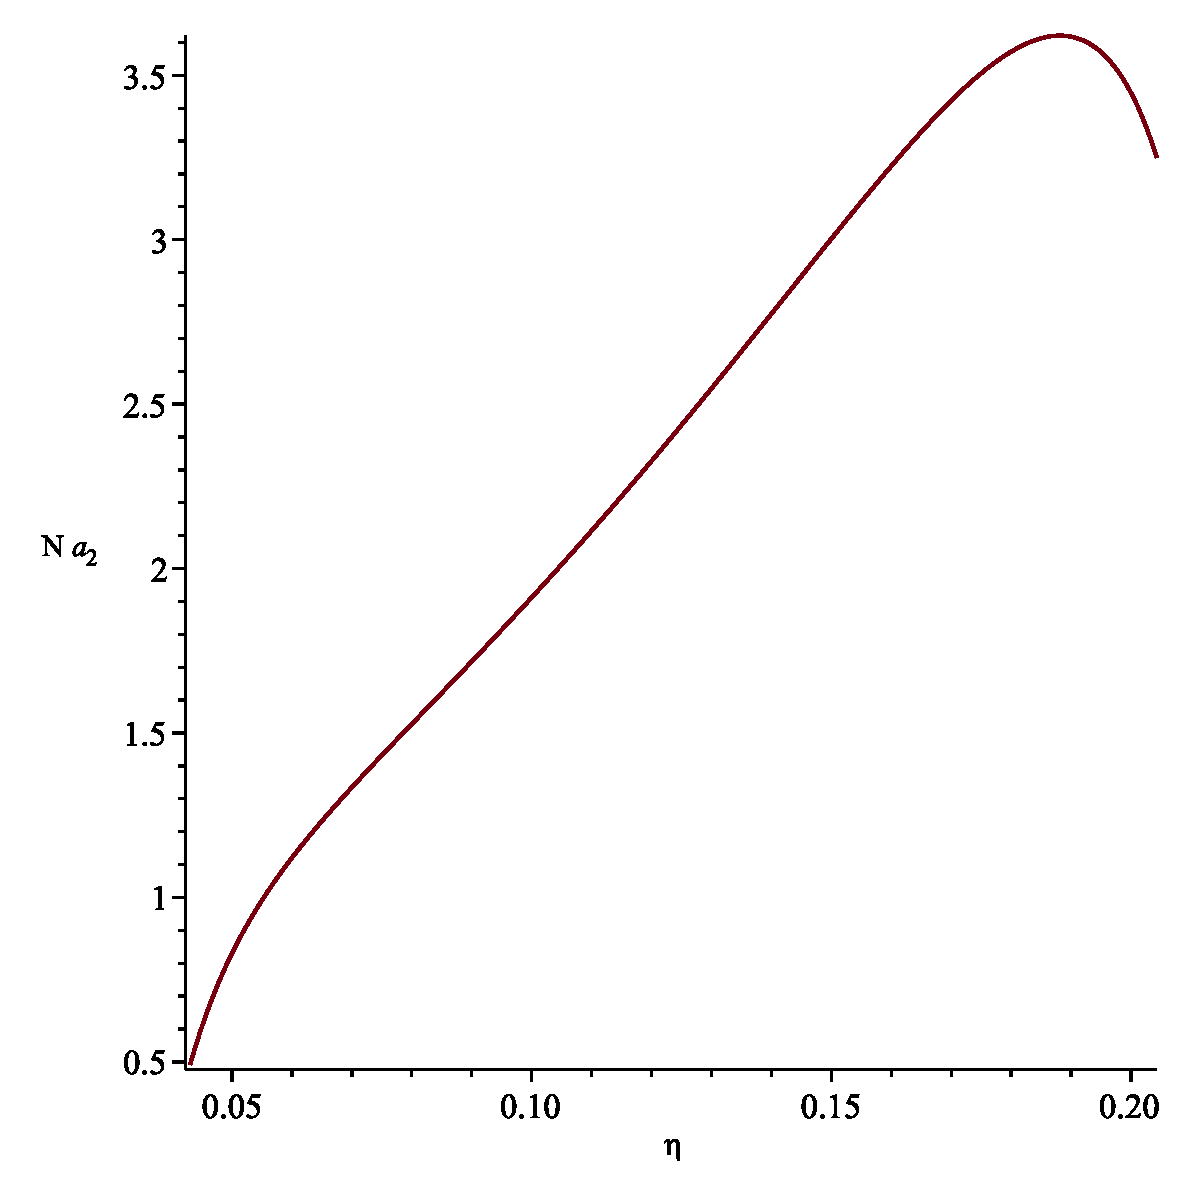
\includegraphics[width=0.45\textwidth,angle=0]{a2_as_function_of_eta} \hfill
	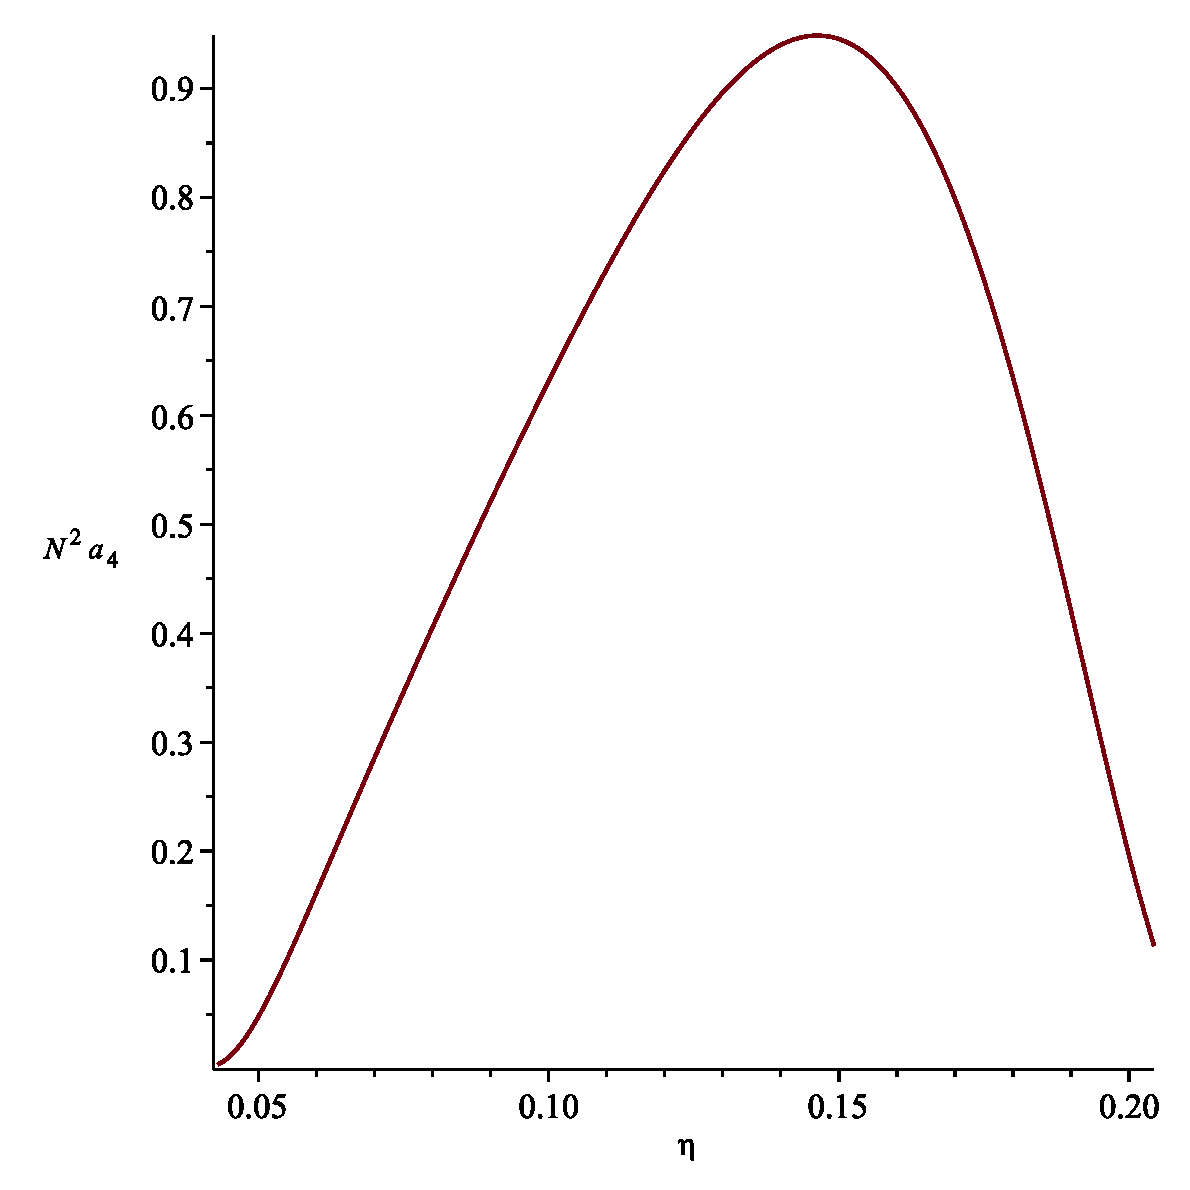
\includegraphics[width=0.45\textwidth,angle=0]{a4_as_function_of_eta} \\
	\parbox{0.5\textwidth}{\caption{\label{fig:a2_vs_eta} Quantity $\langle N \rangle_0 a_2$ as a function of $\eta$ for $R_0/\alpha=3.5$.
	}} \hfill
	\parbox{0.45\textwidth}{\caption{\label{fig:a4_vs_eta} Quantity $\langle N \rangle_0^2 a_4$ as a function of $\eta$ for $R_0/\alpha=3.5$.
	}}
\end{figure}

To rewrite $d(k)$ in a useful form, let's first consider the quantity $\alpha(k)$
\begin{equation}
	\alpha(k) = \frac{\beta \hat{\Phi}_k}{V} = \frac{1}{\langle N \rangle_0} \frac{6}{\pi}\eta \frac{\varepsilon}{k_B T} \frac{\hat{\Phi}_k}{\varepsilon\sigma^3}.
\end{equation}
It is seen now that the quantity $\langle N \rangle_0 d(k)$ is a function of $\eta$, but also depends on the parameter of the interaction potential $\Phi$, as well as on the temperature $T$. 
\section{Effective Hamiltonian in the mean-field approximation}
Consider the long-wave contribution $\Xi_L$ to the GPF, Eq.~(\ref{Xi_L}). Let's calculate $\Xi_L$ in the approximation when all $\vb k_i=0$
\begin{equation}
	\Xi_L^{(1)} = \int \exp(\mu^*\rho_0 -\frac{d(0)}{2} \rho_0^2 - \frac{a_4}{4!N_B} \rho_0^4) {\rm d} \rho_0.
\end{equation}
Since, as previously learned, $d(0) \propto \langle N \rangle_0$ and $a_4 \propto \langle N \rangle_0^2$, it is convenient to perform the following substitution of variables $\rho = \langle N \rangle_0 \rho_0'$ in the the above expression and obtain
\begin{equation}
	\Xi_L^{(1)} = \langle N \rangle_0 \int \exp[\langle N \rangle_0 E(\rho'_0)] {\rm d} \rho'_0
\end{equation}
where the following notations were introduced
\begin{equation}
	E(\rho'_0) = \mu^*\rho_0' - \frac{d'(0)}{2} {\rho'}_0^2 - \frac{a'_4}{4!}{\rho'}_0^4,
\end{equation}
\begin{equation}
	d'(0) = \langle N \rangle_0 d(0) = a'_2 + \frac{6}{\pi}\eta \frac{\varepsilon}{k_BT} \frac{\hat{\Phi}_0}{\varepsilon\sigma^3}.
\end{equation}
\begin{equation}
	a'_2 = \langle N \rangle_0 a_2, \quad a'_4 = \frac{\langle N \rangle_0}{N_B} \langle N \rangle_0^2 a_4
\end{equation}
The presence of $\langle N \rangle_0$ in the exponent justifies the application of the steepest-descent method for integration. The result is the following
\begin{equation}
	\label{mf:Xi_L_1}
	\Xi_L^{(1)} = \langle N \rangle_0 \exp(\langle N \rangle_0 E(\rho_{0,{\rm max}}))
\end{equation}
where $\rho_{0,{\rm max}}$ maximizes the quantity $E(\rho'_0)$ and is found from the following conditions
\begin{equation}
	\frac{\partial E}{\partial \rho'_0} = 0; \quad \frac{\partial^2 E}{\partial {\rho'}_0^2} < 0.
\end{equation}
In explicit form these conditions become
\begin{equation}
	\label{eq_rho_mean_field}
	\mu^*-d'(0)\rho_0 - \frac{a'_4}{3!}{\rho'}_0^3 = 0,
\end{equation}
\begin{equation}
	-d'(0) - \frac{a'_4}{2}{\rho'}_0^2 < 0.
\end{equation}

\subsection{Naive approximation}
In the most simple approximation, the quantity $\mu^*$ plays the same role as an external magnetic field in the Ising model. For Ising model it is known that the critical point appears at the absence of the external field, thus to find the critical point in our approximation, one condition is 
$$\mu^*=0.$$ 
The quantity $\mu^*$ depends on the chemical potential, through the term $\beta(\mu - \mu_0)$, on the temperature, through the term proportional to $\alpha(0)$, and on the packing fraction $\eta.$
If we assume that $\mu = \mu_0$, then the condition $\mu^*=0$ will relate the temperature and $\eta$
$$
{\frak M_3}/{\frak M_4} + \alpha(0)\tilde{\frak M}_1 = 0.
$$


This is the first condition that relates these two quantities.
The second condition is obtained from the requirement that non-zero solution exists for $\rho'_0$:
$$ {\rho'}^3_0 + \frac{3!d'(0)}{a'_4}{\rho'}_0 = 0 $$

$$
\rho_{01} = 0;
$$ 

$$
\rho_{02,03} = \pm\sqrt{-\frac{3!d'(0)}{a'_4}}
$$

Since $a'_4$ is always positive in the region $0.04 \leq \eta \leq 0.22$, the solutions $\rho_{02}$ and $\rho_{03}$ are real when $d'(0) \leq 0$. Thus the second condition for the critical point is 
$$
d'(0) = 0
$$

Thus in explicit form the system of two equations relating the temperature and packing fraction is as follows
\begin{eqnarray}
	&&\frac{\mathfrak{m}_3}{\mathfrak{m}_4} + \frac{6\eta}{\pi} \frac{1}{T^*} \frac{\hat{\Phi}_0}{\varepsilon\sigma^3}
	\left(1 - \frac{\mathfrak{m}_2\mathfrak{m}_3}{\mathfrak{m}_4} + \frac{\mathfrak{m}_3^3}{3\mathfrak{m}_4^2} \right) = 0;
	\nonumber\\
	&& a'_2 + \frac{6\eta}{\pi} \frac{1}{T^*} \frac{\hat{\Phi}_0}{\varepsilon\sigma^3} = 0,
\end{eqnarray}
where $T^* = k_BT/\varepsilon$ is the reduced temperature.
The equation for finding the critical value of $\eta$ is 
\begin{equation}
	\frac{\mathfrak{m}_3}{\mathfrak{m}_4} - a'_2
	\left(1 - \frac{\mathfrak{m}_2\mathfrak{m}_3}{\mathfrak{m}_4} + \frac{\mathfrak{m}_3^3}{3\mathfrak{m}_4^2} \right) = 0.
\end{equation}
\begin{figure}[htbp]
	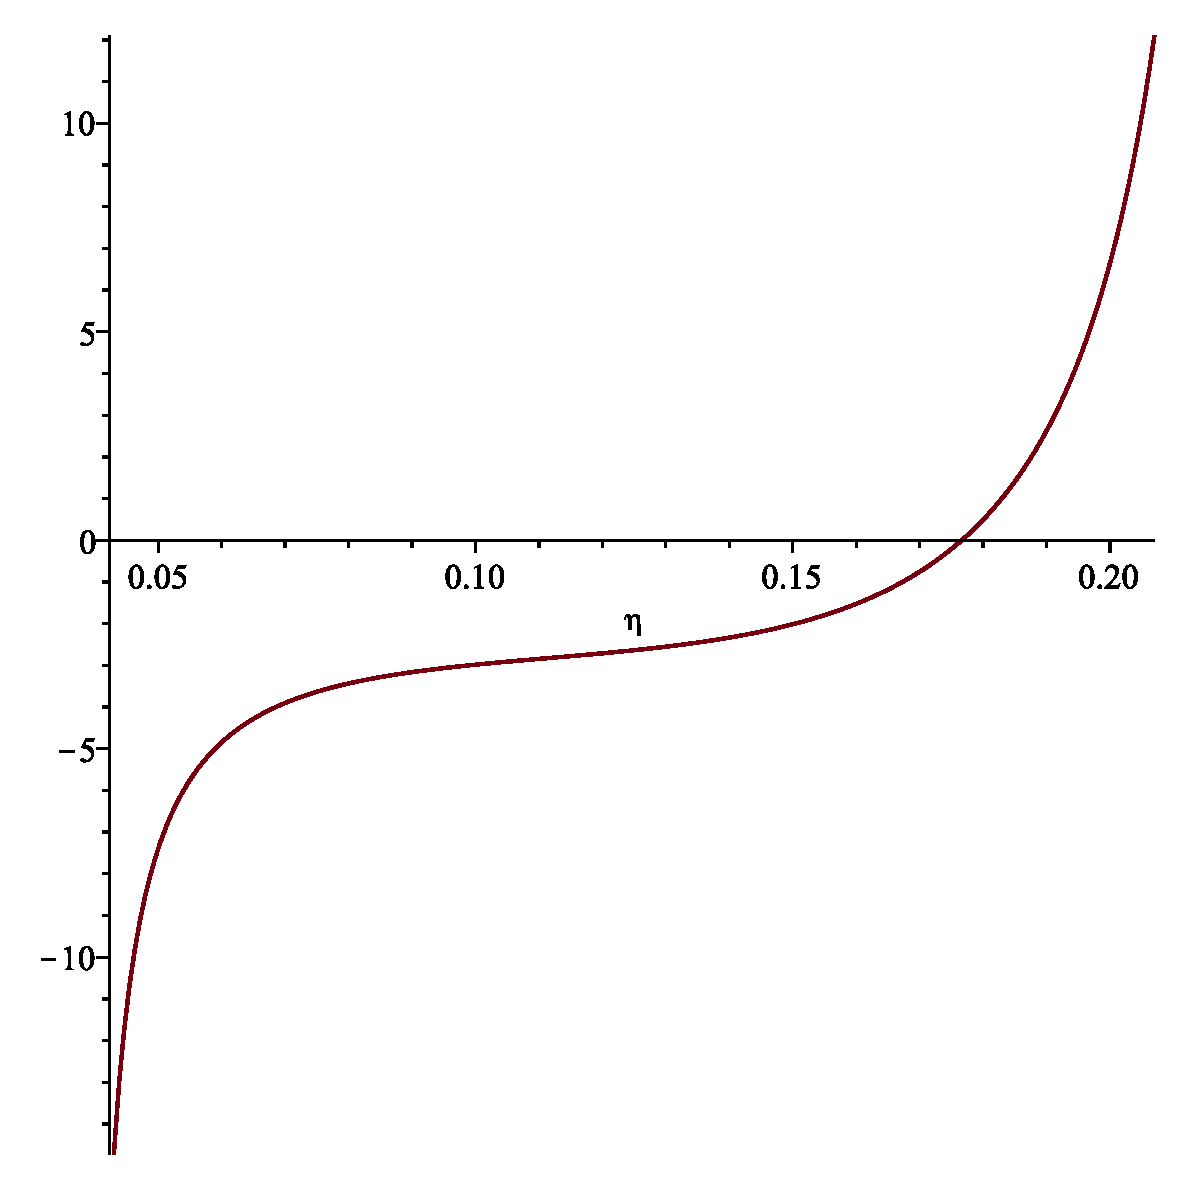
\includegraphics[width=0.7\textwidth,angle=0]{equation_for_critical_density}
	\caption{Equation for the critical value of the packing fraction $\eta_c$.}
	\label{eq_for_eta_c}
\end{figure}
Figure~\ref{eq_for_eta_c} shows this equation graphically. The numerical solution to the equation gives the following value in the Percus-Yevick approximation
$$
\eta_c = 0.1742,
$$
or the critical value for the reduced density $\rho^* = \sigma^3\langle N \rangle / V$
$$
\rho^*_c = 0.3327.
$$
In the Carnahan-Starling approximation the corresponding values are
\begin{equation}
	\eta_c = 0.1766, \quad \rho^*_c = 0.3374.
\end{equation}
The critical temperature is now found
$$
T^*_c = -\frac{6\eta_c}{\pi a'_2} \frac{\hat{\Phi}_0}{\varepsilon\sigma^3}
$$
which for the parameters value $R_0/\alpha = 3.5$ is $T^*_c=2.14$ in Percus-Yevick approximation, and $T^*_c=2.15$ in the Carnahan-Starling one.
It is very important to note that both critical density and critical temperature depend on the parameters of the attractive part of potential. In particular, the critical temperature $T_c$ approaches zero as the interaction potential becomes more and more narrow ($\alpha \to \infty,$ $\hat{\Phi}_0 \to 0$).

The solutions to the equation~(\ref{eq_rho_mean_field}) for $\rho'_0$ can be written in general form via the discriminant of this cubic equation (via the Cardano's formulas). We are not going to do so for this simple approximation, but are going to integrate expression~(\ref{Xi_L}) over non-zero values of $k$, obtain similar equation for $\rho_0$ but with re-normalized coefficients, and investigate the obtained equation more closely.

\subsection{Applying condition $\langle N \rangle_0 = \langle N \rangle$}
Another way to address the problem of finding the critical point coordinates is to impose the condition of equality between particle numbers averages for the reference system and the whole system
\begin{equation}
	\langle N \rangle_0 = \langle N \rangle.
\end{equation}
This condition was, for example, applied in~\cite{YukhJSP1995}.

The general equation to find the average (equilibrium) number of particles is
\begin{equation}
	\left(\frac{\partial \ln\Xi}{\partial (\beta\mu)}\right)_{T,V} = \langle N \rangle.
\end{equation}
In the expression~\ref{Xi_as_prod} for the grand partition function $\Xi$ only $\Xi_L$ depends on the chemical potential. Taking into account its expression~\ref{Xi_L}, as well as the expression~\ref{mf:Xi_L_1} for $\Xi_L^{(1)}$, we arrive at the equation
\begin{equation}
	\langle N \rangle_0
	\left(
	\mathfrak{m}_1 + \frac{\mathfrak{m}_2 \mathfrak{m}_3}{\abs{\mathfrak{m}_4}} + \frac{\mathfrak{m}_3^3}{3\mathfrak{m}_4^2}  + \rho_0^{\rm{max}}
	\right) 
	= \langle N \rangle.
\end{equation}
Applying the conditions $\langle N \rangle_0 = \langle N \rangle$ and $\mathfrak{m}_1 = 1$, we get
\begin{equation}
	\rho_0^{\rm{max}} = - \left(\frac{\mathfrak{m}_2 \mathfrak{m}_3}{\abs{\mathfrak{m}_4}} + \frac{\mathfrak{m}_3^3}{3\mathfrak{m}_4^2}\right).
\end{equation}
In a number of works, see e.g.~\cite{YukhJSP1995,Yukh2013,Yukh2014}, the right-hand side expression is considered as a distinct quantity and is denoted as $\Delta$
\begin{equation}
	\label{def:Delta}
	\Delta \equiv - \left(\frac{\mathfrak{m}_2 \mathfrak{m}_3}{\abs{\mathfrak{m}_4}} + \frac{\mathfrak{m}_3^3}{3\mathfrak{m}_4^2}\right).
\end{equation}

Thus there are three conditions to be met at the critical point. The first one, which follows from the requirements of Ising model symmetry, is
\begin{eqnarray}
	\mu^* = 0.
\end{eqnarray}
The second one is
\begin{equation}
	d'(0) = 0,
\end{equation}
and the third one, which follows from the requirement that $\rho_0^{\rm{max}} = 0$ at the critical point, is
\begin{equation}
	\Delta = 0.
\end{equation}
From the last condition we can immediately find the value of the critical density. Solving the equation $\Delta = 0$ numerically gives us 
\begin{equation}
	\eta_c = 0.12867, \quad \rho^*_c = 0.24574
\end{equation}
in the Percus-Yevick approximation, and
\begin{equation}
	\eta_c = 0.13044, \quad \rho^*_c = 0.24913
\end{equation}
in the Carnahan-Starling approximation.
It worth noting that the condition $\Delta = 0$ is equivalent to $\mathfrak{M}_3=0$, and consequently to $\mathfrak{m}_3 = 0.$

The equation for the critical temperature follows from the second condition
\begin{equation}
	\label{T_c_Delta}
	T^*_c = -\frac{6\eta_c}{\pi a'_2} \frac{\hat{\Phi}_0}{\varepsilon\sigma^3} = -\frac{\rho^*_c}{a'_2} \frac{\hat{\Phi}_0}{\varepsilon\sigma^3}.
\end{equation}
Its numerical values for the potential parameter $R_0/\alpha = 3.5$ are $T^*_c=2.197$ and $T^*_c=2.202$ in the Percus-Yevick and Carnahan-Starling approximations, respectively.

There are a few important conclusions regarding results based on the condition $\langle N \rangle_0 = \langle N \rangle$. First, the value of the critical density does not depend on the parameters of the attractive part of the potential. This consequence is very contradictory since the critical density is the same for any form of $\Phi(r)$ at $r\geq \sigma$, including very weak interactions. 
The value of $\eta_c$ does not depend on the approximation used for the grand partition function calculation, and its mean-field value obtained in this work is the same as the one obtained in~\cite{YukhJSP1995}.

Second, the critical temperature does depend on the parameters of interaction, and approaches zero as the range of interaction becomes shorter and shorter ($\alpha \to \infty,$ $\hat{\Phi}_0 \to 0$).

In this approach we can also find the value of the chemical potential at the critical point. From the condition $\mu^*=0$ and Eq.~(\ref{mu_star}) we get
$$
	\beta(\mu_c - \mu_0) = -\mathfrak{M}_3/\mathfrak{M}_4 - \alpha(0)\tilde{\mathfrak{M}}_1 
	= -\mathfrak{m}_3/\mathfrak{m}_4 - \frac{6\eta}{\pi} \frac{\varepsilon}{k_{\rm{B}}T} \frac{\hat{\Phi}_0}{\varepsilon\sigma^3} \tilde{\mathfrak{m}}_1
$$
where the following notation was introduced by the analogy with Eq.~(\ref{def:tilde_M_1})
\begin{equation}
	\tilde{\mathfrak{m}}_1 = \mathfrak{m}_1 -\frac{\mathfrak{m}_2 \mathfrak{m}_3}{\mathfrak{m}_4} + \frac{\mathfrak{m}_3^3}{3\mathfrak{m}_4^2},
\end{equation}
Since $\mathfrak{m}_3 = 0$ at the critical point, and $\mathfrak{m}_1 = 1$, we get
\begin{equation}
	\beta(\mu_c - \mu_0) = -\frac{\rho^*_c}{T^*_c} \frac{\hat{\Phi}_0}{\varepsilon\sigma^3} = a'_2.
\end{equation}
The numerical values of the chemical potential difference at the critical point are summarized in Table~\ref{tab:critical_chem_potential} for different interaction parameters.

\begin{table}[h]
	\caption{Critical values of chemical potential for different parameters $R_0/\alpha$.}
	\label{tab:critical_chem_potential}
	\begin{center}
		\begin{tabular}{|c|c|c|}
			%\begin{tabular}{cccccccccc}
			\hline
			$R_0/\alpha$ \quad & $\beta(\mu_c - \mu_0)$ \quad & $\beta\mu^{\rm{ex}}_c$ \quad \quad \\
			\hline
			2.0  & 2.6699 & 4.0342 \\
			2.5  & 2.6228 & 3.9872 \\
			3.0  & 2.5812 & 3.9456 \\
			3.5  & 2.5453 & 3.9097 \\
			4.0  & 2.5143 & 3.8787 \\
			4.5  & 2.4877 & 3.8520 \\
			5.0  & 2.4645 & 3.8289 \\
			5.5  & 2.4444 & 3.8088 \\
			6.0  & 2.4268 & 3.7911 \\
			\hline
		\end{tabular}
	\end{center}
\end{table}

The chemical potential of a system can be represented as a sum of ideal and excess parts
$$
	\mu = \mu^{\rm{id}} + \mu^{\rm{ex}}.
$$
Thus the difference $\beta(\mu - \mu_0)$ is essentially the difference between excess chemical potentials. The excess chemical potential of a hard-sphere system in the Carnahan-Starling approximation is
\begin{equation}
	\beta\mu^{\rm{ex}}_0 = \frac{8\eta - 9\eta^2 + 3\eta^3}{(1-\eta)^3}.
\end{equation}
At the critical density $(\beta\mu^{\rm{ex}}_0)_c = 1.3644$. Thus, we can calculate the excess chemical potential of the whole system at the critical point. The results are presented in Table~\ref{tab:critical_chem_potential}.


\appendix
\section{\label{sec:total_corr_func} Total correlation functions}
\subsection{Definitions}
The definition of the n-particle distribution function is taken from \cite{HANSEN2013ch2} (see Eq.~(2.6.7) therein)
\begin{equation}
\label{def:g_n}
g^{(n)}(\vb{r}^n)=\frac{\rho^{(n)}(\vb{r}_1,\dotsc,\vb{r}_n)}{\prod_{i=1}^{n}\rho^{(1)}(\vb{r}_i)}
\end{equation}
where $\rho^{(n)}$ is the n-particle density (see Eq.~(2.6.1) in \cite{HANSEN2013ch2}), which is defined as:
\begin{eqnarray}
	\label{def:rho_n}
	\rho^{(n)}(\vb r^n) = \frac{1}{\Xi}\sum_{N=n}^{\infty} \frac{z^N}{(N-n)!} \int\exp(-\beta U_N) d\vb r^{(N-n)}
\end{eqnarray}
Here $\vb r^n \equiv \vb r_1, \dotsc, \vb r_n$, and $d\vb r^{(N-n)} = d\vb r_{n+1} \dotsc d\vb r_N$.

Let's introduce an hierarchy of total correlation functions. The most widely known element of this hierarchy is the pair correlation function
\begin{equation}
\label{def:pair_corr_func}
h^{(2)}(\vb{r}_1,\vb{r}_2) = g^{(2)}(\vb{r}_1,\vb{r}_2) - 1
\end{equation}
(e.g., see Eq.~(2.6.8) in~\cite{HANSEN2013ch2}).

Let's express the total correlation functions in terms of the n-particle distribution functions.
Formally, one can introduce the hierarchy of total correlation functions starting from $n=1$ and on.
By definition
\begin{equation}
g^{(1)}(\vb{r})\equiv 1.
\end{equation}
Thus, for $n=1$ one has: 
\begin{equation}
h^{(1)}(\vb{r}) = g^{(1)}(\vb{r}) = 1.
\end{equation}

For $n=2$:
\begin{equation}
h^{(2)}(\vb{r}_1,\vb{r}_2) = g^{(2)}(\vb{r}_1,\vb{r}_2) - 1
\end{equation}

For $n=3$:
\begin{eqnarray}
h^{(3)}(\vb{r}_1 ,\vb{r}_2, \vb{r}_3) &=& g^{(3)}(\vb{r}_1, \vb{r}_2, \vb{r}_3) - g^{(2)}(\vb{r}_1, \vb{r}_2) 
\nonumber\\
&&-g^{(2)}(\vb{r}_1,\vb{r}_3) -  g^{(2)}(\vb{r}_2,\vb{r}_3) +2.
\end{eqnarray}

For $n=4$ :
\begin{eqnarray}
h^{(4)}(\vb{r}_1, \vb{r}_2, \vb{r}_3, \vb{r}_4) &=& g^{(4)}(\vb{r}_1, \vb{r}_2, \vb{r}_3, \vb{r}_4) - g^{(3)}(\vb{r}_1, \vb{r}_2, \vb{r}_3) 
\nonumber\\
&&-g^{(3)}(\vb{r}_1, \vb{r}_2, \vb{r}_4) -  g^{(3)}(\vb{r}_1, \vb{r}_3, \vb{r}_4) - g^{(3)}(\vb{r}_2, \vb{r}_3, \vb{r}_4) 
\nonumber\\
&&-g^{(2)}(\vb{r}_1,\vb{r}_2) g^{(2)}(\vb{r}_3,\vb{r}_4) - g^{(2)}(\vb{r}_1,\vb{r}_3) g^{(2)}(\vb{r}_2,\vb{r}_4) - g^{(2)}(\vb{r}_1,\vb{r}_4)g^{(2)}(\vb{r}_2,\vb{r}_3)
\nonumber\\
&&+2(g^{(2)}(\vb{r}_1,\vb{r}_2) + g^{(2)}(\vb{r}_1,\vb{r}_3) + g^{(2)}(\vb{r}_1,\vb{r}_4)
\nonumber\\
&&+g^{(2)}(\vb{r}_2,\vb{r}_3) + g^{(2)}(\vb{r}_2,\vb{r}_4) + g^{(2)}(\vb{r}_3,\vb{r}_4)) 
\nonumber\\
&&-6.
\end{eqnarray}

\subsection{Expressed via $g^{(n)}$ and $h^{(m<n)}$}
The total correlation functions $h^{(n)}$ can be expressed via $g^{(n)}$ and $h^{(m<n)}$.
Such representation for total correlation functions $h^{(3)}$ and $h^{(4)}$ was used in \cite{attardJCP1990}.

For $n=3$:
\begin{eqnarray}
h^{(3)}(\vb{r}_1 ,\vb{r}_2, \vb{r}_3) &=& g^{(3)}(\vb{r}_1, \vb{r}_2, \vb{r}_3) - h^{(2)}(\vb{r}_1, \vb{r}_2) 
\nonumber\\
&&-h^{(2)}(\vb{r}_1,\vb{r}_3) -  h^{(2)}(\vb{r}_2,\vb{r}_3) -1.
\end{eqnarray}

For $n=4$:
\begin{eqnarray}
h^{(4)}(\vb{r}_1, \vb{r}_2, \vb{r}_3, \vb{r}_4) &=& g^{(4)}(\vb{r}_1, \vb{r}_2, \vb{r}_3, \vb{r}_4) - h^{(3)}(\vb{r}_1, \vb{r}_2, \vb{r}_3) 
\nonumber\\
&&-h^{(3)}(\vb{r}_1, \vb{r}_2, \vb{r}_4) -  h^{(3)}(\vb{r}_1, \vb{r}_3, \vb{r}_4) - h^{(3)}(\vb{r}_2, \vb{r}_3, \vb{r}_4) 
\nonumber\\
&&-h^{(2)}(\vb{r}_1,\vb{r}_2) h^{(2)}(\vb{r}_3,\vb{r}_4) - h^{(2)}(\vb{r}_1,\vb{r}_3) h^{(2)}(\vb{r}_2,\vb{r}_4) - h^{(2)}(\vb{r}_1,\vb{r}_4)h^{(2)}(\vb{r}_2,\vb{r}_3)
\nonumber\\
&&-h^{(2)}(\vb{r}_1,\vb{r}_2) - h^{(2)}(\vb{r}_1,\vb{r}_3) - h^{(2)}(\vb{r}_1,\vb{r}_4)
\nonumber\\
&&-h^{(2)}(\vb{r}_2,\vb{r}_3) - h^{(2)}(\vb{r}_2,\vb{r}_4) - h^{(2)}(\vb{r}_3,\vb{r}_4) 
\nonumber\\
&&-1.
\end{eqnarray}

From here it's straightforward to express $g^{(n)}$ via $h^{(m)}$, where $m \leq n$ (in \cite{hernandoPRA1986} such expressions were presented for $n\leq3$).

\subsection{Expressed via $g^{(n)}$ through $g^{(1)}$}
For $n=2$:
\begin{eqnarray}
h^{(2)}(\vb{r}_1,\vb{r}_2) = g^{(2)}(\vb{r}_1,\vb{r}_2) - g^{(1)}(\vb{r}_1) g^{(1)}(\vb{r}_2)
\end{eqnarray}

For $n=3$:
\begin{eqnarray}
h^{(3)}(\vb{r}_1 ,\vb{r}_2, \vb{r}_3) &=& g^{(3)}(\vb{r}_1, \vb{r}_2, \vb{r}_3) - g^{(2)}(\vb{r}_1, \vb{r}_2) g^{(1)}(\vb{r}_3)
\nonumber\\
&&-g^{(2)}(\vb{r}_1,\vb{r}_3) g^{(1)}(\vb{r}_2) -  g^{(2)}(\vb{r}_2,\vb{r}_3) g^{(1)}(\vb{r}_1)
\nonumber\\
&& +2g^{(1)}(\vb{r}_1)g^{(1)}(\vb{r}_2)g^{(1)}(\vb{r}_3).
\end{eqnarray}

For $n=4$ :
\begin{eqnarray}
h^{(4)}(\vb{r}_1, \vb{r}_2, \vb{r}_3, \vb{r}_4) &=& g^{(4)}(\vb{r}_1, \vb{r}_2, \vb{r}_3, \vb{r}_4) - g^{(3)}(\vb{r}_1, \vb{r}_2, \vb{r}_3) g^{(1)}(\vb{r}_4)
\nonumber\\
&&-g^{(3)}(\vb{r}_1, \vb{r}_2, \vb{r}_4) g^{(1)}(\vb{r}_3) -  g^{(3)}(\vb{r}_1, \vb{r}_3, \vb{r}_4) g^{(1)}(\vb{r}_2) - g^{(3)}(\vb{r}_2, \vb{r}_3, \vb{r}_4)g^{(1)}(\vb{r}_1) 
\nonumber\\
&&-g^{(2)}(\vb{r}_1,\vb{r}_2) g^{(2)}(\vb{r}_3,\vb{r}_4) - g^{(2)}(\vb{r}_1,\vb{r}_3) g^{(2)}(\vb{r}_2,\vb{r}_4) - g^{(2)}(\vb{r}_1,\vb{r}_4)g^{(2)}(\vb{r}_2,\vb{r}_3)
\nonumber\\
&& + 2[g^{(2)}(\vb{r}_1,\vb{r}_2)g^{(1)}(\vb{r}_3) g^{(1)}(\vb{r}_4) + g^{(2)}(\vb{r}_1,\vb{r}_3) g^{(1)}(\vb{r}_2) g^{(1)}(\vb{r}_4) 
\nonumber\\
&& + g^{(2)}(\vb{r}_1,\vb{r}_4)g^{(1)}(\vb{r}_2)g^{(1)}(\vb{r}_3) + g^{(2)}(\vb{r}_2,\vb{r}_3)g^{(1)}(\vb{r}_2) g^{(1)}(\vb{r}_4)
\nonumber\\
&& + g^{(2)}(\vb{r}_2,\vb{r}_4)g^{(1)}(\vb{r}_1) g^{(1)}(\vb{r}_3) + g^{(2)}(\vb{r}_3,\vb{r}_4)g^{(1)}(\vb{r}_1) g^{(1)}(\vb{r}_2) ]
\nonumber\\
&&-6g^{(1)}(\vb{r}_1) g^{(1)}(\vb{r}_2)g^{(1)}(\vb{r}_3) g^{(1)}(\vb{r}_4).
\end{eqnarray}

Equivalent representations for n-point correlation functions were used in \cite{white1979} in research on galaxy clustering.

To simplify notation, let's denote $(\vb{r}_1, \dotsc, \vb{r}_n) = (1, \dotsc, n)$. And let's group similar terms under summation sings.
Then $h^{(3)}$ and $h^{(4)}$ can be rewritten as
\begin{eqnarray}
h^{(3)}(1,2,3) &=& g^{(3)}(1, 2, 3) 
- \sum_{\vb l = \left\{\substack{1,2,3 \\ 1,3,2 \\ 2,3,1} \right\} } g^{(2)}(l_1,l_2) g^{(1)}(l_3)
\nonumber\\
&& +2g^{(1)}(1)g^{(1)}(2)g^{(1)}(3).
\end{eqnarray}
\begin{eqnarray}
h^{(4)}(1,2,3,4) &=& g^{(4)}(1,2,3,4) 
- \sum_{\vb l = \left\{\substack{1,2,3,4 \\ 1,2,4,3 \\ 1,3,4,2 \\ 2,3,4,1}\right\} }g^{(3)}(l_1,l_2,l_3) g^{(1)}(l_4) 
\nonumber\\
&&-\sum_{\vb l = \left\{ \substack{1,2,3,4 \\ 1,3,2,4 \\ 1,4,2,3} \right\}}g^{(2)}(l_1,l_2) g^{(2)}(l_3,l_4)
\nonumber\\
&& + 2\sum_{\vb l = \left\{\substack{1,2,3,4 \\ 1,3,2,4 \\ 1,4,2,3 \\ 2,3,1,4 \\ 2,4,1,3 \\ 3,4,1,2} \right\}} g^{(2)}(l_1,l_2)g^{(1)}(l_3) g^{(1)}(l_4) 
\nonumber\\
&&-6g^{(1)}(1) g^{(1)}(2)g^{(1)}(3) g^{(1)}(4).
\end{eqnarray}

The sums extend over all distinct argument lists in which each point appears exactly once. E.g. $g^{(3)}(1,2,3)$ and $g^{(3)}(3,2,1)$ are not considered distinct, and terms such as $g^{(2)}(1,2)g^{(2)}(2,3)$ do not appear \cite{white1979}.

\subsection{Fourier components of total correlation functions}
The following generic notation is used for the Fourier components of the total correlation function:
\begin{equation}
\hat{h}^{(n)}(\vb{k}_1,\dotsc, \vb{k}_n) = \int \exp(-i\vb{k}_1\vb{r}_1 - \dotsc - i\vb{k}_n\vb{r}_n) h^{(n)}(\vb{r}_1, \dotsc, \vb{r}_n) d\vb{r}_1\dotsc d\vb{r}_n
\end{equation}
By properly selecting the origin, it can be shown that for a homogeneous isotropic system:
\begin{equation}
g^{(n)}(\vb{r}_1, \dotsc, \vb{r}_n) = g^{(n)}(\vb{r}_1 - \vb{r}_n, \dotsc, \vb{r}_{n-1} - \vb{r}_{n})
\end{equation}
and applying a proper change of variables it can be written as:
\begin{equation}
g^{(n)} = g^{(n)}(\vb{r}_1, \dotsc, \vb{r}_{n-1})
\end{equation}
Thus,
\begin{equation}
h^{(n)}(\vb{r}_1, \dotsc, \vb{r}_n) \Rightarrow h^{(n)}(\vb{r}_1, \dotsc, \vb{r}_{n-1})
\end{equation}

It enables us to write the following expressions for the Fourier components $\hat{h}^{(n)} (\vb{k}^n)$:
\begin{equation}
\frac{1}{V}\hat{h}^{(n)} (\vb{k}^n) = \hat{h}^{(n)} (\vb{k}_1, \dotsc, \vb{k}_{n-1}) 
\delta_{\vb{k}_1+\dotsc + \vb{k}_n}
\end{equation}
where
\begin{equation}
\hat{h}^{(n)}(\vb{k}_1, \dotsc, \vb{k}_{n-1}) = \int \exp(-i\vb{k}_1\vb{r}_1 - \dotsc - i\vb{k}_{n-1}\vb{r}_{n-1}) h^{(n)}(\vb{r}_1, \dotsc, \vb{r}_{n-1})d\vb{r}_1\dotsc d\vb{r}_{n-1}
\end{equation}

In particular, for $n=1$:
\begin{equation}
\hat{h}^{(1)}(\vb{k}) = \int \exp(-i\vb{k}\vb{r})h^{(1)}(\vb{r})d\vb{r} = \int \exp(-i\vb{k}\vb{r})d\vb{r}
\end{equation}
\begin{equation}
\frac{1}{V}\hat{h}^{(1)}(\vb{k}) = \delta_{\vb{k}}
\end{equation}

For $n=2$:
\begin{equation}
\frac{1}{V}\hat{h}^{(2)}(\vb{k}_1, \vb{k}_2) = \hat{h}^{(2)}(\vb{k}_1)\delta_{\vb{k}_1 + \vb{k}_2}
\end{equation}

\subsection{Fourier transform of the radial correlation function for the hard-spheres system}
From~\cite{Ashcroft1966} (see Eqs.~(3)-(5) therein) an explicit expression for $\hat{h}^{(2)}(k)$ can be calculated in the Percus-Yevick approximation.
Figure~\ref{h2_vs_k} shows the dependency of $\hat{h}^{(2)}(k)/\sigma^3$ on $k \sigma$. Figure~\ref{h2_vs_eta} shows the dependency of $\hat{h}^{(2)}(0)/\sigma^3$ on packing fraction $\eta.$
\begin{figure}[htbp]
	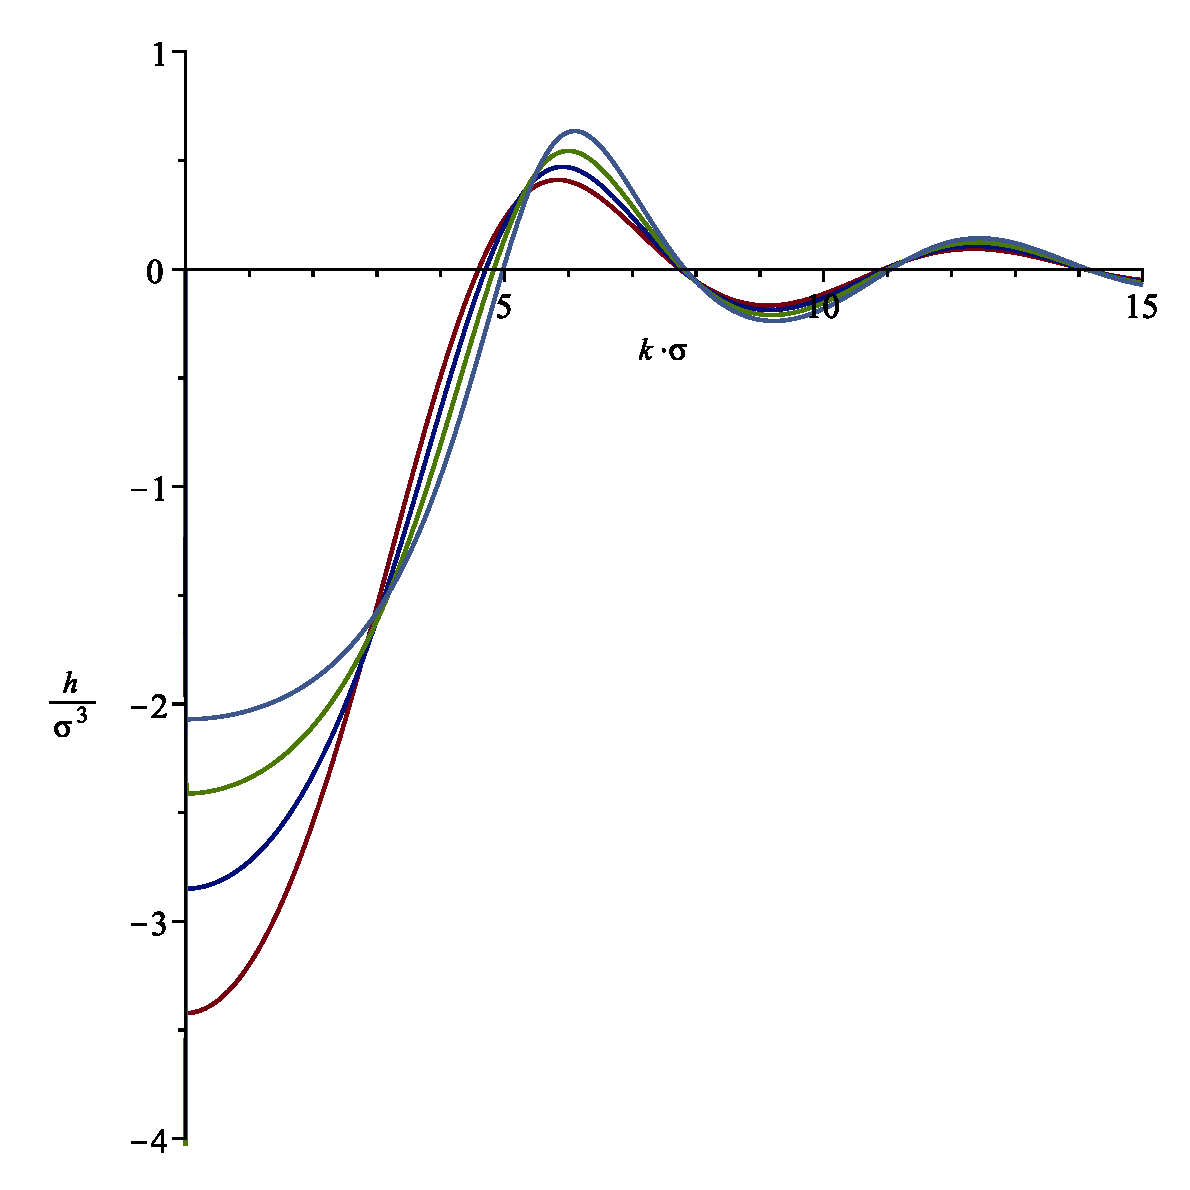
\includegraphics[width=0.45\textwidth,angle=0]{h2_as_function_of_k_at_different_eta} \hfill
	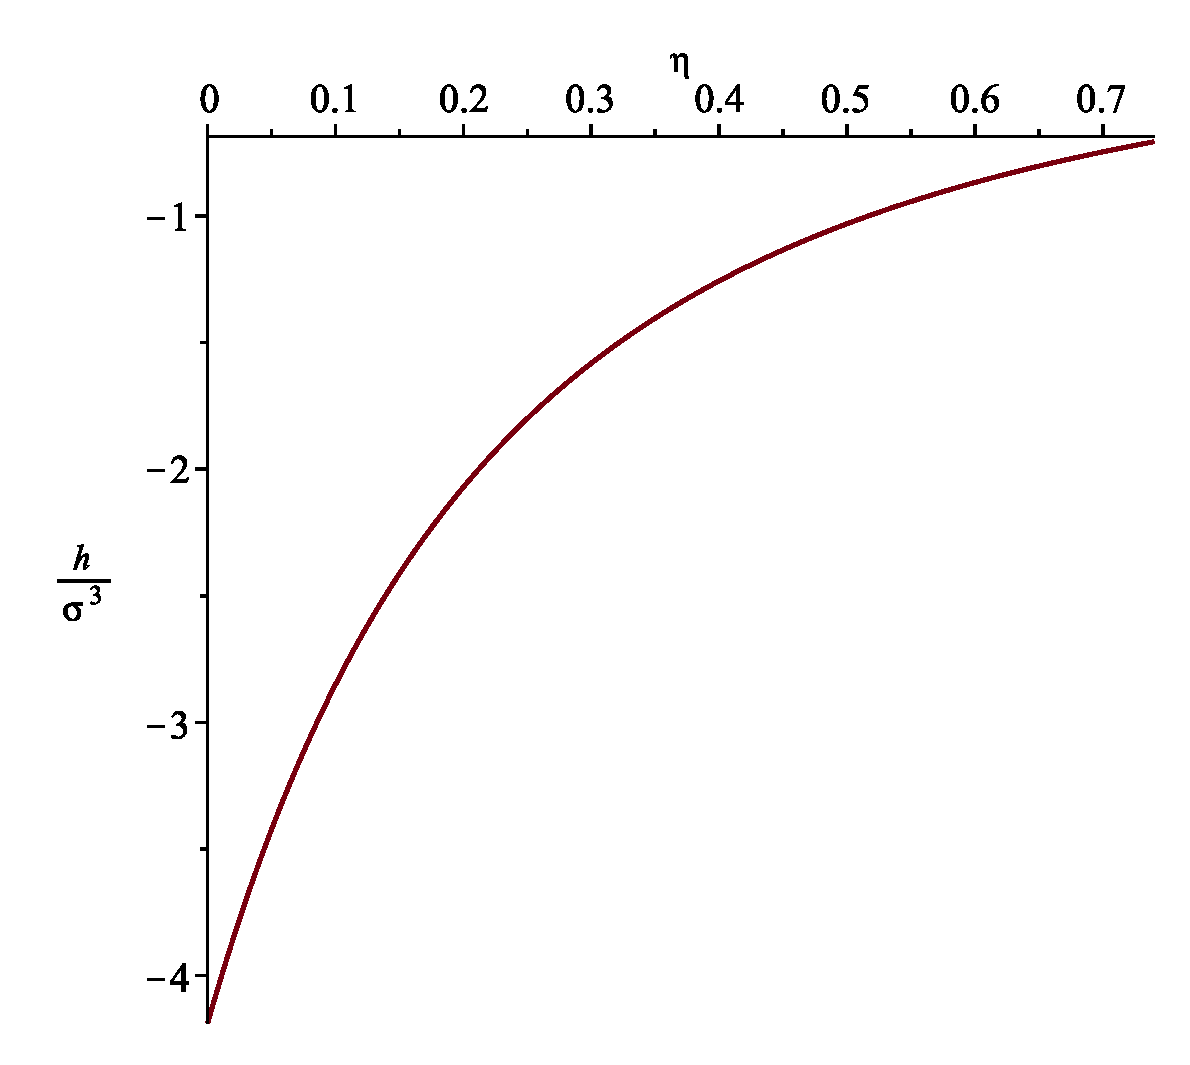
\includegraphics[width=0.45\textwidth,angle=0]{h2_as_function_of_eta_at_k_equals_0} \\
	\parbox{0.5\textwidth}{\caption{\label{h2_vs_k} Fourier transform of the total correlation function $\hat{h}^{(2)}(k)$ divided by the cube of HS diameter $\sigma$ as a function of $k\sigma$ at different values of packing fraction $\eta$. $\eta = 0.05$, $\eta=0.1$, $\eta = 0.15$, and $\eta=0.2$.
	}} \hfill
	\parbox{0.45\textwidth}{\caption{\label{h2_vs_eta} Fourier transform of the total correlation function $\hat{h}^{(2)}(k)$ divided by the cube of HS diameter $\sigma$ as a function of packing fraction $\eta$ at $\vb k = 0$
	}}
\end{figure}

\subsection{Some recurrence relations for correlation functions}
In this section, some recurrence relations for the total correlation functions $h^{(n)}$ will be derived. Let's use equations for the $n$-particle density from~\cite{Schofield1966} (Eq.~(A7) therein):
\begin{equation}
	\frac{\partial\rho^{(n)}}{\partial\rho}\bigg|_T = \frac{n\rho^{(n)} 
		+ \int \{ \rho^{(n+1)}(\vb r_1, \dotsc, \vb r_{n+1}) - \rho^{(n)}(\vb r_1, \dotsc, \vb r_n) \rho^{(1)}(\vb r_{n+1}) \} {\rm d} \vb r_{n+1}}
	{(1/V)\int \rho^{(1)}(\vb r_1) {\rm d} \vb r_1 + \int \{ \rho^{(2)}(\vb r_1, \vb r_2) - \rho^{(1)}(\vb r_1)\rho^{(1)}(\vb r_2) \} {\rm d} \vb r_1}
\end{equation}
which is rewritten in terms of the $n$-particle distribution functions as (Eq.~(A8) in~\cite{Schofield1966})
\begin{equation}
	\label{recur_g}
	\frac{\partial (\rho^n g^{(n)})}{\partial\rho} \bigg|_T 
	= \frac{n\rho^{n-1}g^{(n)} + \rho^n \int \{g^{(n+1)}(\vb r_1, \dots, \vb r_{n+1}) - g^{(n)}(\vb r_1, \dots, \vb r_n)\} {\rm d} \vb r_{n+1}}
	{1 + \rho\int \{g^2(\vb r_1, \vb r_2) - 1\} {\rm d} \vb r_1}
\end{equation}

First, consider $n=2$ and rewrite~(\ref{recur_g}) in terms of correlation functions:
\begin{eqnarray}
	&&\frac{\partial}{\partial\rho}\left(\rho^2 h^{(2)}(\vb r_1, \vb r_2) + \rho^2\right) =
	\nonumber\\
	&&= \frac
	{2\rho(h^{(2)}(\vb r_1, \vb r_2) + 1) + \int \left(h^{(3)}(\vb r_1, \vb r_2, \vb r_3) + h^{(2)}(\vb r_1, \vb r_3) + h^{(2)}(\vb r_2, \vb r_3) \right) {\rm d}{\vb r_3}}
	{1 + \rho \hat{h}^{(2)}(0)}.
\end{eqnarray}
Then apply the following Fourier transformation to the above equation:
\begin{equation}
	\mathcal{F}_2(\dots) = \iint {\rm e}^{-{\rm i}\vb k_1 \vb r_1 - {\rm i} \vb k_2 \vb r_2} \dots {\rm d} \vb r_1 {\rm d} \vb r_2
\end{equation}
As a result, after some algebraic manipulations, the following relations between $\hat{h}^{(3)}$ and $\hat{h}^{(2)}$ are obtained:
\begin{equation}
	\hat{h}^{(3)}(\vb k_1, \vb k_2, 0) = 2 \hat{h}^{(2)}(0)\hat{h}^{(2)}(\vb k_1, \vb k_2) + \frac{\partial \hat{h}^{(2)}(\vb k_1, \vb k_2)}{\partial\rho}(1 + \rho\hat{h}^{(2)}(0)),
\end{equation}
\begin{equation}
	\label{recur_h3_h2}
	\hat{h}^{(3)}(k, -k) = 2 \hat{h}^{(2)}(0)\hat{h}^{(2)}(k) + \frac{\partial \hat{h}^{(2)}(k)}{\partial\rho}(1 + \rho\hat{h}^{(2)}(0)).
\end{equation}

Similarly, the relations between $\hat{h}^{(4)}$ and $\hat{h}^{(3)}$ are as following:
\begin{equation}
	\hat{h}^{(4)}(\vb k_1, \vb k_2, \vb k_3, 0) = 3\hat{h}^{(2)}(0)\hat{h}^{(3)}(\vb k_1, \vb k_2, \vb k_3) + \frac{\partial \hat{h}^{(3)}(\vb k_1, \vb k_2, \vb k_3)} {\partial \rho} (1 + \rho\hat{h}^{(2)}(0)),
\end{equation}
\begin{equation}
	\label{recur_h4_h3}
	\hat{h}^{(4)}(\vb k_1, \vb k_2, 0) = 3\hat{h}^{(2)}(0)\hat{h}^{(3)}(\vb k_1, \vb k_2) + \frac{\partial \hat{h}^{(3)}(\vb k_1, \vb k_2)} {\partial \rho} (1 + \rho\hat{h}^{(2)}(0))
\end{equation}
The relations~(\ref{recur_m3_m2}) and~(\ref{recur_m4_m2}) for cumulants follow directly from~(\ref{recur_h3_h2}) and~(\ref{recur_h4_h3}), respectively.


\section{\label{app:cumulant_calc}Cumulants calculation}
For the sake of simplicity, in this Appendix we will omit the subscript $0$ at the notation for averages, $\langle\dotsc\rangle_0 \Rightarrow  \langle\dotsc\rangle$, and also will understand $\Psi_N \equiv\Psi_N(\vb r^N)$.
\subsection{$n=1$}
\begin{equation}
	\mathfrak{M}_1(\vb k) = \langle \hat{\rho}_{\vb k} \rangle.
\end{equation}
\begin{eqnarray}
	\langle \hat{\rho}_{\vb k} \rangle &=& \Xi_0^{-1} \sum_{N=0}^{\infty} \frac{z_0^N}{N!} \int \sum_{j=1}^N \exp(-{\rm i}\vb k\vb r_j) \exp(-\beta\Psi_N) {\rm d} {\vb r}^N 
	\nonumber\\
	&=&\Xi_0^{-1} \sum_{N=0}^{\infty} \frac{z_0^N}{N!} \int \exp(-{\rm i}\vb k\vb{r}') \sum_{j=1}^N \delta(\vb r' - \vb r_j) \exp(-\beta\Psi_N) {\rm d} {\vb r}^N {\rm d}{\vb r'}
	\nonumber\\
	&=&\int \exp(-{\rm i}\vb k\vb{r}') \left\langle \sum_{j=1}^N \delta(\vb r' - \vb r_j) \right\rangle {\rm d}{\vb r'}
\end{eqnarray}
From \cite{HANSEN2013ch2} (see Eq~(2.5.11) and the last paragraph on p.40 therein)
\begin{equation}
	\left\langle \sum_{j=1}^N \delta(\vb r' - \vb r_j) \right\rangle = \rho^{(1)}(\vb r')
\end{equation}
where $\rho^{(1)}(\vb r)$ is the equilibrium singe-particle density.

For homogeneous system (uniform fluid):
\begin{equation}
	\rho^{(1)}(\vb r) = \frac{\langle N\rangle}{V}
\end{equation}
Thus
\begin{equation}
	\langle \hat{\rho}_{\vb k} \rangle = \frac{\langle N\rangle }{V} \int \exp(-{\rm i}\vb k \vb r') {\rm d} \vb r' = \langle N\rangle \delta_{\vb k}.
\end{equation}
\begin{equation}
	\boxed{
		\mathfrak{M}_1(\vb k) = \langle N\rangle \delta_{\vb k}.
	}
\end{equation}

\subsection{$n=2$}
\begin{equation}
	\mathfrak{M}_2(\vb k_1, \vb k_2)
	= \langle \hat{\rho}_{\vb k_1} \hat{\rho}_{\vb k_2} \rangle - \langle \hat{\rho}_{\vb k_1} \rangle \langle\hat{\rho}_{\vb k_2} \rangle
\end{equation}
\begin{equation}
	\langle \hat{\rho}_{\vb k} \rangle = \langle N\rangle \delta_{\vb k}.
\end{equation}
\begin{eqnarray}
	\langle \hat{\rho}_{\vb k_1} \hat{\rho}_{\vb k_2} \rangle &=& \Xi_0^{-1} \sum_{N=0}^{\infty} \frac{z_0^N}{N!} \int 
	\sum_{i=1}^N \exp(-{\rm i}\vb k_1\vb r_i) \sum_{j=1}^N \exp(-{\rm i}\vb k_2\vb r_j) \exp(-\beta\Psi_N) {\rm d} {\vb r}^N
\end{eqnarray}
Let's single out the term with $i=j$:
\begin{eqnarray}
	\langle \hat{\rho}_{\vb k_1} \hat{\rho}_{\vb k_2} \rangle &=& 
	\Xi_0^{-1} \sum_{N=0}^{\infty} \frac{z_0^N}{N!} \int 
	\left[
	\sum_{i=1}^N \exp(-{\rm i}(\vb k_1 +  \vb k_2)\vb r_i)
	\right. \nonumber\\
	&& \left. + \sum_{i=1}^N \exp(-{\rm i}\vb k_1\vb r_i) \sum_{j=1 \atop j\neq i}^N \exp(-{\rm i}\vb k_2\vb r_j) 
	\right]\exp(-\beta\Psi_N) {\rm d} {\vb r}^N
\end{eqnarray}
The first term is $\langle\hat{\rho}_{\vb k_1 + \vb k_2} \rangle$ and thus is equal to $\langle N \rangle\delta_{\vb k_1 + \vb k_2}$.
Let's rewrite the second term via $\delta$-functions:
\begin{eqnarray}
	\langle \hat{\rho}_{\vb k_1} \hat{\rho}_{\vb k_2} \rangle &=& \langle N \rangle\delta_{\vb k_1 + \vb k_2}
	\nonumber\\
	&+& \Xi_0^{-1} \sum_{N=0}^{\infty} \frac{z_0^N}{N!} \int 
	{\rm e}^{-{\rm i}\vb k_1\vb r'} {\rm e}^{-{\rm i}\vb k_2\vb r''} 
	\sum_{i=1}^N  \sum_{j=1 \atop j\neq i}^N \delta(\vb r'- \vb r_i) \delta(\vb r'' - \vb r_j)
	\exp(-\beta\Psi_N) {\rm d} {\vb r}^N {\rm d} {\vb r'} {\rm d} {\vb r''}
	\nonumber\\
	&=& 
	\langle N \rangle\delta_{\vb k_1 + \vb k_2} + \iint {\rm e}^{-{\rm i}\vb k_1\vb r'} {\rm e}^{-{\rm i}\vb k_2\vb r''}  
	\left\langle \sum_{i=1}^N  \sum_{j=1 \atop j\neq i}^N \delta(\vb r'- \vb r_i) \delta(\vb r'' - \vb r_j) \right\rangle {\rm d} {\vb r'} {\rm d} {\vb r''}
\end{eqnarray}
From \cite{HANSEN2013ch2} (see Eq~(2.5.13) and the last paragraph on p.40 therein) it follows
\begin{equation}
	\left\langle \sum_{i=1}^N  \delta(\vb r'- \vb r_i) \sum_{j=1 \atop j\neq i}^N \delta(\vb r'' - \vb r_j) \right\rangle = \rho^{(2)}(\vb r', \vb r'')
\end{equation}
where $\rho^{(2)}(\vb r', \vb r'')$ is the equilibrium 2-particle density, or just the pair density
\begin{eqnarray}
	\langle \hat{\rho}_{\vb k_1} \hat{\rho}_{\vb k_2} \rangle &=& \langle N \rangle\delta_{\vb k_1 + \vb k_2} + 
	\iint {\rm e}^{-{\rm i}\vb k_1\vb r'} {\rm e}^{-{\rm i}\vb k_2\vb r''}  
	\rho^{(2)}(\vb r', \vb r'') {\rm d} {\vb r'} {\rm d} {\vb r''}.
\end{eqnarray}
Taking into account the definition~(\ref{def:g_n}) of the $n$-particle distribution function $g^{(n)}$, and the relationship between $\rho^{(n)}$ and $g^{(n)}$ for a homogeneous system
\begin{equation}
	\rho^{(n)}(\vb r^n) = \rho^n g^{(n)}(\vb r^n)
\end{equation}
where $\rho = \langle N \rangle / V$ is the particle density, one arrives at
\begin{eqnarray}
	\langle \hat{\rho}_{\vb k_1} \hat{\rho}_{\vb k_2} \rangle &=& \langle N \rangle\delta_{\vb k_1 + \vb k_2} + 
	\rho^2 \iint {\rm e}^{-{\rm i}\vb k_1\vb r'} {\rm e}^{-{\rm i}\vb k_2\vb r''}  
	g^{(2)}(\vb r', \vb r'') {\rm d} {\vb r'} {\rm d} {\vb r''}.
\end{eqnarray}
Here $g^{(2)}(\vb r', \vb r'')$ is called the pair distribution function.
Taking into account the definition~(\ref{def:pair_corr_func}) for the pair (total) correlation function $h^{(2)}$, one has
\begin{eqnarray}
	\langle \hat{\rho}_{\vb k_1} \hat{\rho}_{\vb k_2} \rangle &=& \langle N \rangle\delta_{\vb k_1 + \vb k_2} + 
	\rho^2 \iint {\rm e}^{-{\rm i}\vb k_1\vb r'} {\rm e}^{-{\rm i}\vb k_2\vb r''}  
	h^{(2)}(\vb r', \vb r'') {\rm d} {\vb r'} {\rm d} {\vb r''}
	\nonumber\\
	&+& \frac{\langle N \rangle^2}{V^2}\iint {\rm e}^{-{\rm i}\vb k_1\vb r'} {\rm e}^{-{\rm i}\vb k_2\vb r''} {\rm d} {\vb r'} {\rm d} {\vb r''}.
\end{eqnarray}
The last term is equal to $\langle N \rangle^2 \delta_{\vb k_1}\delta_{\vb k_2}.$ 
For isotropic system $h^{(2)}(\vb r', \vb r'') = h^{(2)}(\abs{\vb r' - \vb r''})$, and the second term becomes
\begin{eqnarray}
	&\frac{\langle N \rangle^2}{V^2} &\iint {\rm e}^{-{\rm i}\vb k_1\vb r'} {\rm e}^{-{\rm i}\vb k_2\vb r''} {\rm d} {\vb r'} {\rm d} {\vb r''} = 
	\left| \substack{\text{Change of variables:} \\ \vb r = \vb r' - \vb r''; \quad \vb R = \vb r'' \\
	\vb r' = \vb R + \vb r; \quad \vb r'' = \vb R \\ {\rm d} \vb r'{\rm d} \vb r'' = {\rm d} \vb r{\rm d} \vb R } 
	\right| 
	\nonumber\\
	&=& \frac{\langle N \rangle^2}{V^2} \int \exp(-{\rm i}(\vb k_1 + \vb k_2)\vb R) {\rm d} \vb R
	\int \exp(-{\rm i}\vb k_1 \vb r) h^{(2)}(r) {\rm d}\vb r
	\nonumber\\
	&=& \frac{\langle N \rangle^2}{V} \hat{h}^{(2)}(\vb k_1) \delta_{\vb{k}_1 + \vb{k}_2} = 
	\langle N \rangle \rho \hat{h}^{(2)}(\vb k_1) \delta_{\vb{k}_1 + \vb{k}_2}.
\end{eqnarray}
One arrives at the final expression for $\langle \hat{\rho}_{\vb k_1} \hat{\rho}_{\vb k_2} \rangle$:
\begin{eqnarray}
	\langle \hat{\rho}_{\vb k_1} \hat{\rho}_{\vb k_2} \rangle &=& \langle N \rangle\delta_{\vb k_1 + \vb k_2} + 
	\langle N \rangle \rho \hat{h}^{(2)}(\vb k_1) \delta_{\vb{k}_1 + \vb{k}_2}
	+ \langle N \rangle^2 \delta_{\vb k_1}\delta_{\vb k_2}
	\nonumber.
\end{eqnarray}
And for the cumulant $\mathfrak{M}_2$ the final expression is
\begin{equation}
	\boxed{
		\mathfrak{M}_2(\vb k_1, \vb k_2) = \langle N \rangle \delta_{\vb{k}_1 + \vb{k}_2} (1 + \rho\hat{h}^{(2)}(\vb 	k_1)) 
	}
\end{equation}

The quantity $1 + \rho \hat{h}^{(2)}(\vb k)$ is equal to the static structure factor of the uniform fluid (see~\cite{HANSEN2013ch2}, Eq.~(3.6.10)):
\begin{equation}
	S(\vb k) = 1 + \hat{h}^{(2)}(\vb k)
\end{equation}
\begin{equation}
	\mathfrak{M}_2(\vb k_1, \vb k_2)  = \langle N \rangle \delta_{\vb{k}_1 + \vb{k}_2} S(\vb k_1).
\end{equation}
The structure factor is related to the thermodynamic properties via the following relationship (see Eqs.~(2.6.12), (3.5.14), and~(3.6.11) in~\cite{hansen2013theory}):
\begin{equation}
	S(0) = 1 + \rho\hat{h}^{(2)}(0) = \rho \chi_T / \beta = \frac{\langle N^2 \rangle - \langle N \rangle^2}{\langle N \rangle},
\end{equation}
where $\chi_T$ is the isothermal compressibility.
Thus for $\vb k_1 = \vb k_2 = 0$:
\begin{equation}
	\boxed{
		\mathfrak{M}_2(0,0) = \langle N^2 \rangle - \langle N \rangle^2
	}
\end{equation}

\section{\label{app:cumulant_calc_k_0}A method of calculation for cumulants at $\vb k_i = 0$}
It follows from~(\ref{def:cumulant}) and~(\ref{def:jacob_tilde}), that 
\begin{eqnarray}
	\mathfrak{M}_n(0, \dotsc, 0) &=& \frac{1}{(-{\rm i}2\pi)^n} \frac{\partial^n \ln \langle\exp(-{\rm i}2\pi \sum_{\vb k} \omega_{\vb k}\hat{\rho}_{\vb k}) \rangle_0}
	{\partial\omega_0^n} \bigg|_{\omega_{\vb k_i} = 0}
	\nonumber\\
	&=& \frac{\partial^n \ln \Xi_0}{\partial(\beta\mu_0)^n} 
	= \frac{\partial^{n-1}\langle N \rangle_0}{\partial(\beta\mu_0)^{n-1}} 
	= \frac{\partial^{n-1}\mathfrak{M}_1(0)}{\partial(\beta\mu_0)^{n-1}}
	\nonumber\\
	&=& \frac{\partial\mathfrak{M}_{n-1}(0,\dotsc,0)}{\partial(\beta\mu_0)}.
\end{eqnarray}
Then from~(\ref{def:average_rs}) one derives
\begin{equation}
	\frac{\partial \langle N \rangle_0}{\partial(\beta\mu_0)} = \langle N^2 \rangle_0 - \langle N \rangle_0^2,
\end{equation}
\begin{equation}
	\frac{\partial \langle N^2 \rangle_0}{\partial(\beta\mu_0)} = \langle N^3 \rangle_0 - \langle N^2 \rangle_0\langle N \rangle_0,
\end{equation}
\begin{equation}
	\frac{\partial \langle N^3 \rangle_0}{\partial(\beta\mu_0)} = \langle N^4 \rangle_0 - \langle N^3 \rangle_0\langle N \rangle_0,
\end{equation}
and so on, to give in general:
\begin{equation}
	\frac{\partial \langle N^n \rangle_0}{\partial(\beta\mu_0)} = \langle N^{n+1} \rangle_0 - \langle N^n \rangle_0\langle N \rangle_0.
\end{equation}
Thus the equation for $\mathfrak{M}_2(0,0)$ is obtained immediately
\begin{eqnarray}
	\mathfrak{M}_2(0,0) &=& \frac{\partial \langle N \rangle_0}{\partial(\beta\mu_0)} = \langle N^2 \rangle_0 - \langle N \rangle_0^2 
	\nonumber\\
	&=& \langle (N - \langle N \rangle_0)^2 \rangle_0. 
\end{eqnarray}
Explicit calculation for $\mathfrak{M}_3(0,0,0)$ leads to
\begin{eqnarray}
	\mathfrak{M}_3(0,0,0) &=& \frac{\partial}{\partial(\beta\mu_0)}\left(\langle N^2 \rangle_0 - \langle N \rangle_0^2\right) 
	\nonumber\\
	&=& \langle N^3 \rangle_0 - \langle N^2 \rangle_0\langle N \rangle_0 - 2\langle N \rangle_0\langle N^2 \rangle_0 + 2\langle N \rangle_0\langle N \rangle_0^2
	\nonumber\\
	&=& \langle N^3 \rangle_0 -3 \langle N^2 \rangle_0\langle N \rangle_0 + 2\langle N \rangle_0^3
	\nonumber\\
	&=& \langle (N - \langle N \rangle_0)^3 \rangle_0.
\end{eqnarray}
And for $\mathfrak{M}_4(0,0,0,0):$
\begin{eqnarray}
	\mathfrak{M}_4(0,0,0,0) &=& \frac{\partial}{\partial(\beta\mu_0)}
	\left(\langle N^3 \rangle_0 - 3\langle N^2 \rangle_0\langle N \rangle_0 +2 \langle N \rangle_0^3\right) 
	\nonumber\\
	&=& \langle N^4 \rangle_0 - \langle N^3 \rangle_0\langle N \rangle_0 
	- 3\left(\langle N^3 \rangle_0 - \langle N^2 \rangle_0\langle N \rangle_0\right)\langle N \rangle_0
	\nonumber\\
	&-&3\langle N^2 \rangle_0 \left(\langle N^2 \rangle_0 - \langle N \rangle_0^2 \right)
	+ 6\langle N \rangle_0^2 \left(\langle N^2 \rangle_0 - \langle N \rangle_0^2\right)
	\nonumber\\
	&=& \langle N^4 \rangle_0 
	- 4\langle N^3 \rangle_0\langle N \rangle_0 
	+ 12\langle N^2 \rangle_0\langle N \rangle_0^2 
	- 3\langle N^2 \rangle_0^2 
	- 6\langle N \rangle_0^4
	\nonumber\\
	&=& \langle (N - \langle N \rangle_0)^4 \rangle_0 - 3 \langle (N - \langle N \rangle_0)^2 \rangle_0^2.
\end{eqnarray}

\section{Critical point coordinates}
This section reports values obtained for the critical point coordinates - critical values for reduced temperature $k_{{\rm B}}T_c / \varepsilon$, packing fraction $\eta_c$, excess chemical potential $\beta(\mu_c - \mu_0)$.

\subsection{Temperature}
\begin{table}[h]
	\caption{Critical temperature values}
	\begin{center}
		\begin{tabular}{|c|c|c|}
			%\begin{tabular}{cccccccccc}
			\hline
			$k_{{\rm B}}T_c / \varepsilon$  \quad & Reference \quad & Details \quad \quad \\
			\hline
			1.31  & \cite{YukhJSP1995} & Ar \\
			2.197  & This work & MF; Percus-Yevick; Morse $R_0/\alpha=3.5$ \\
			2.202  & This work & MF; Carnahan-Starling; Morse $R_0/\alpha=3.5$ \\
			\hline
		\end{tabular}
	\end{center}
\end{table}


\subsection{Density}

\begin{table}[h]
	\caption{Critical density values}
	\begin{center}
		\begin{tabular}{|c|c|c|c|}
			%\begin{tabular}{cccccccccc}
			\hline
			$\eta$  \quad & $\rho^*$ \quad & Reference \quad & Details \quad \quad \\
			\hline
			0.130443  & 0.249128 & \cite{YukhJSP1995} & Carnahan-Starling; $\langle N \rangle_{RS} = \langle N \rangle$ \\
			0.13044  & 0.24913 & This work & MF; Carnahan-Starling; \\
			0.12867  & 0.24574 & This work & MF; Percus-Yevick; \\
			\hline
		\end{tabular}
	\end{center}
\end{table}

\subsection{Chemical potential}
See Table~\ref{tab:critical_chem_potential}

\section{\label{sec:fourier} Fourier transformation}
In this work, the following form of Fourier transformation is used.

Let $f(\vb r)$ be a function of the distance $\vb r$. Then it is expanded in the Fourier series as:
\begin{equation}
	f(\vb r) = \frac{1}{V} \sum_{\vb k} \hat{f}_{\vb k} e^{i\vb k \vb r}
\end{equation}
where $\sum_{\vb k} = \sum_{k_x}\sum_{k_y}\sum_{k_z}$, $k_i = \frac{2\pi}{V^{1/3}}n_i$, $i=x,y,z$, $n_i=0,\pm 1, \pm 2, \dotsc$. $V$ is the volume of periodicity.

The expression for the Fourier component $\hat{f}_{\vb k}$ is
\begin{equation}
	\hat{f}_{\vb k} = \int_V f(\vb r) e^{-i\vb k \vb r} d{\vb r}.
\end{equation}

Note, that here we agree upon the convention that the $'+'$ sign is taken in the exponent when $f(\vb r)$ is expressed via $\hat{f}_{\vb k}$, and the $'-'$ sign when $\hat{f}_{k}$ is expressed via $f(\vb r)$.

\subsection*{Expression of $\delta$-function}

I.
\begin{equation}
	\delta(\vb r - \vb r') = \frac{1}{(2\pi)^3}\int d {\vb k} e^{i\vb k (\vb r - \vb r')} = \frac{1}{V} \sum_{\vb k} e^{i\vb k(\vb r - \vb r')}.
\end{equation}

\begin{equation}
	\int f(\vb r) \delta(\vb r - \vb r') d {\vb r} = f(\vb r').
\end{equation}

II.
\begin{equation}
	\delta(\vb k - \vb k') = \frac{1}{(2\pi)^3} \int d{\vb r} e^{i\vb r (\vb k - \vb k')}
\end{equation}

\begin{equation}
	\int d{\vb k} \hat{f}_{\vb k} \delta(\vb k - \vb k') = \frac{(2\pi)^3}{V} \sum_{\vb k} \hat{f}_{\vb k} \delta(\vb k - \vb k') = \hat{f}_{\vb k'}.
\end{equation}

Relations between integration and summation over $\vb k$ is given by
\begin{equation}
	\frac{1}{V}\sum_{\vb k} (...) = \frac{1}{(2\pi)^3}\int d{\vb k} (...)
\end{equation}

\subsection*{Kronecker's $\delta$-symbol}

\begin{equation}
	\delta_{\vb k} = \frac{1}{V} \int e^{-i\vb k \vb r} d{\vb r} = 
	\left\{
	\begin{array}{cc}
		0, \quad \vb k \neq 0, \\
		1, \quad \vb k = 0.
	\end{array}
	\right.
\end{equation}

\begin{equation}
	\delta_{\vb k, \vb k'} = \frac{1}{V} \int e^{-i(\vb k - \vb k') \vb r} d{\vb r} = 
	\left\{
	\begin{array}{cc}
		0, \quad \vb k \neq \vb k', \\
		1, \quad \vb k = \vb k'.
	\end{array}
	\right.
\end{equation}
\section{Notation}
$\vb r$ - the coordinate in three-dimensional space;

$r \equiv \abs{\vb r}$ - the absolute value of $\vb r$.

$\vb k$ - the wave vector in the reciprocal space.

$k \equiv \abs{\vb k}$ - the absolute value of the wave vector $\vb k$.

$\delta(...)$ - the Dirac's $\delta$-function.

$\delta_{...}$ - the Kronecker's $\delta$-symbol.

$V$ - the volume.

$N$ - the number of particles.

$\rho$ - the particle density.

$\eta$ - the packing fraction.

$n(\vb r)$ - the microscopic particle density.

$\hat{\rho}_{\vb k}$ - the Fourier component of the microscopic particle density.

$\rho_{\vb k},$ $\rho_0$ - the collective variables.

$\Xi$ - the grand partition function.

$z$ - the activity.

$\mu$ - the chemical potential.

$\Xi_0,$ $z_0,$ $\mu_0$ - the grand partition function, activity, and chemical potential of the reference system, respectively.

$Z_N$ - the configuration integral.

$\beta$ - the inverse temperature.

$\Lambda$ - the de Broglie thermal wavelength.

$\rho^{(n)}(\vb r^n)$ - the equilibrium $n$-particle density.

$g^{(n)}(\vb r^n)$ - the $n$-particle distribution function.

$h^{(n)}(\vb r^n)$ - the $n$-particle total correlation function.

$\hat{h}^{(n)}(\vb k^n)$ - the Fourier component of the $n$-particle total correlation function.

$U(r_{ij})$ - the full pairwise interaction potential between two particles $i$ and $j$ at distance $r_{ij}$.

$U_N(\vb r^N)$, $U_N$ - the potential energy of the interparticle interaction.

$\Psi(r_{ij})$ - the repulsive part of the full interaction potential.

$\Psi_N(\vb r^N)$, $\Psi_N$ - the potential energy of the short-range repulsive interaction.

$\Phi(r_{ij})$ - the attractive part of the full interaction potential. 

$\Phi_N(\vb r^N)$, $\Phi_N$ - the potential energy of the long-range attractive interaction.

$\sigma$ - the hard-sphere diameter. 

$J(\rho - \hat{\rho})$ - the Jacobian for tranformation from $\hat{\rho}_{\vb k}$ to $\rho_{\vb k}.$

$\omega_{\vb k},$ $\omega_0$ - the variables conjugate to collective variables $\rho_{\vb k},$ $\rho_0.$

$\mathfrak{M}_n(\vb k^n),$ $\mathfrak{m}_n(\vb k^{n-1})$ - the cumulants (semi-invariants).

$\mathfrak{J}(\rho)$ - the Jacobian $J(\rho - \hat{\rho})$ averaged over the reference system.

$\tilde{\mathfrak{J}}(\omega)$ - the part of Jacobian $\mathfrak{J}(\rho)$ dependent on $\omega_{\vb k}.$

\section*{Abbreviations}

GPF - Grand Partition Function.

HS - Hard Spheres

RS - Reference System

\tableofcontents

% If in two-column mode, this environment will change to single-column
% format so that long equations can be displayed. Use
% sparingly.
%\begin{widetext}
% put long equation here
%\end{widetext}

% figures should be put into the text as floats.
% Use the graphics or graphicx packages (distributed with LaTeX2e)
% and the \includegraphics macro defined in those packages.
% See the LaTeX Graphics Companion by Michel Goosens, Sebastian Rahtz,
% and Frank Mittelbach for instance.
%
% Here is an example of the general form of a figure:
% Fill in the caption in the braces of the \caption{} command. Put the label
% that you will use with \ref{} command in the braces of the \label{} command.
% Use the figure* environment if the figure should span across the
% entire page. There is no need to do explicit centering.

% \begin{figure}
% \includegraphics{}%
% \caption{\label{}}
% \end{figure}

% Surround figure environment with turnpage environment for landscape
% figure
% \begin{turnpage}
% \begin{figure}
% \includegraphics{}%
% \caption{\label{}}
% \end{figure}
% \end{turnpage}

% tables should appear as floats within the text
%
% Here is an example of the general form of a table:
% Fill in the caption in the braces of the \caption{} command. Put the label
% that you will use with \ref{} command in the braces of the \label{} command.
% Insert the column specifiers (l, r, c, d, etc.) in the empty braces of the
% \begin{tabular}{} command.
% The ruledtabular enviroment adds doubled rules to table and sets a
% reasonable default table settings.
% Use the table* environment to get a full-width table in two-column
% Add \usepackage{longtable} and the longtable (or longtable*}
% environment for nicely formatted long tables. Or use the the [H]
% placement option to break a long table (with less control than 
% in longtable).
% \begin{table}%[H] add [H] placement to break table across pages
% \caption{\label{}}
% \begin{ruledtabular}
% \begin{tabular}{}
% Lines of table here ending with \\
% \end{tabular}
% \end{ruledtabular}
% \end{table}

% Surround table environment with turnpage environment for landscape
% table
% \begin{turnpage}
% \begin{table}
% \caption{\label{}}
% \begin{ruledtabular}
% \begin{tabular}{}
% \end{tabular}
% \end{ruledtabular}
% \end{table}
% \end{turnpage}

% Specify following sections are appendices. Use \appendix* if there
% only one appendix.
%\appendix
%\section{}

% If you have acknowledgments, this puts in the proper section head.
%\begin{acknowledgments}
% put your acknowledgments here.
%\end{acknowledgments}

% Create the reference section using BibTeX:
%\bibliography{basename of .bib file}
%\bibliographystyle{longbibliography}
\bibliography{fluids_cv,fluids_general,correlation_functions,books_romanik_bibliography,online_urls}
%\bibliography{correlation_functions,books_romanik_bibliography}

\end{document}
%
% ****** End of file apstemplate.tex ******

